\documentclass[10pt]{article}
\usepackage{graphicx} % Required for inserting images
\usepackage[utf8]{inputenc}
\usepackage[english]{babel}
\usepackage{amsmath}
\usepackage{amssymb}
\usepackage{amsthm}
\usepackage{mathtools}
\usepackage{float}
\usepackage{subcaption}
\usepackage{caption}
\usepackage{booktabs}
\usepackage{multirow}
\usepackage{array}
\usepackage{xcolor}
\usepackage{geometry}
\usepackage{longtable}
\usepackage{tikz}
\usepackage{pgfplots}
\usepackage{enumitem}
\usepackage{tcolorbox}
\usepackage{wrapfig}
\usepackage{natbib}
\tcbuselibrary{breakable, skins}
\newtcolorbox{keyresult}[1][Key Result]{
  colback=blue!5!white, colframe=blue!60!black,
  title=#1, fonttitle=\bfseries, breakable}
\pgfplotsset{compat=1.18}
\geometry{margin=1in}
\geometry{margin=0.7in}
\begin{document}
\begin{titlepage}
    \begin{center}
        
        % University Logo
        \includegraphics[width=0.3\textwidth]{isi logo.png}\\[1cm]
        
        % Institute Name
        \textsc{\Large Indian Statistical Institute}\\[0.5cm]
        \textsc{\large M.STAT, $2^{nd}$ Semester }\\[1cm]
        
        % Title
        \rule{\linewidth}{0.5mm}\\[0.4cm]
        {\huge \bfseries 2 Sample Location Problem}\\[0.4cm]
        \rule{\linewidth}{0.5mm}\\[1cm]
        
        % Project Type
        \textsc{\large Project Report for Non-parametric Inference}\\[0.5cm]
        
        % Submitted by
        \textsc{\large Submitted by}\\[0.5cm]
        
        % Student Name and Roll Number
        {\large \textbf{Aniv Mazumder (MD2505)}}\\
        {\large \textbf{Koushan Saha (MD2513)}}\\
        {\large \textbf{Sanjhali Parmar (MD2521)}}\\
        [1cm]
        
        % Under the guidance of
        \textsc{\large Under the guidance of}\\[0.5cm]
        
        % Supervisor Name
        {\large \textbf{Advisor}}\\
        {\large Prof. Isha Dewan}\\
        [1cm]
        
        % Date
        {\large March, 2026}\\[1cm]
        
    \end{center}
\end{titlepage}

\tableofcontents
\newpage
\section{Testing Problem}
The \textbf{Two-Sample Location Problem} involves determining whether two independent samples come from populations with the same central tendency (e.g., mean or median). This is typically addressed by testing whether one population is shifted in location relative to the other.
\subsection{Formal Setup}
\begin{enumerate}
    \item \textbf{Data Representations:} \\
    Let $X_1, X_2, \dots, X_m$ be a random sample of size $m$ from a population with a continuous distribution function $F(x)$. Let $Y_1, Y_2, \dots, Y_n$ be a second independent random sample of size $n$ from a population with distribution function $G(x)$. 
    \item \textbf{Location Shift Model:}\\
    We assume the \textit{Location Shift Model} defined as:
    \[ G(x) = F(x - \theta) \]
    where $\theta$ represents the parameter for the shift in location.
    \item \textbf{Hypothesis Testing Setups:}\\
The problem can be formulated in three equivalent ways depending on the level of abstraction:

\begin{enumerate}
    \item \textbf{Setup 1: Parametric Shift Formulation}\\
    Assuming $G(x) = F(x - \theta)$, we test the shift parameter:
    \begin{itemize}
        \item $H_0: \theta = 0$ (No location shift)
        \item $H_1: \theta > 0$ (Rightward shift)
        \item $H_2: \theta < 0$ (Leftward shift)
        \item $H_3: \theta \neq 0$ (Any location shift)
    \end{itemize}

    \item \textbf{Setup 2: Distributional Formulation}\\
    Comparing the cumulative distribution functions directly:
    \begin{itemize}
        \item $H_0: F(x) = G(x) \text{ for all } x$
        \item $H_1: G(x) \leq F(x) \text{ for all } x \text{ (with strict inequality for some } x)$
        \item $H_2: G(x) \geq F(x) \text{ for all } x \text{ (with strict inequality for some } x)$
        \item $H_3: F(x) \neq G(x) \text{ for some } x$
    \end{itemize}

    \item \textbf{Setup 3: Stochastic Ordering Formulation}\\
    Focusing on the probabilistic behavior of the random variables:
    \begin{itemize}
        \item $H_0: X \overset{d}{=} Y$ (Identical in distribution)
        \item $H_1: X \prec_{st} Y$ ($Y$ is stochastically larger than $X$, i.e., $P(Y > a) \geq P(X > a)$)
        \item $H_2: Y \prec_{st} X$ ($X$ is stochastically larger than $Y$)
        \item $H_3: X \overset{d}{\neq} Y$ (Stochastically different)
    \end{itemize}
\end{enumerate}
\end{enumerate}

\subsection{Mann-Whitney U and Wilcoxon Rank Sum Statistic}
Let $X_1, \dots, X_m$ and $Y_1, \dots, Y_n$ be independent random samples of sizes $m$ and $n$ from continuous distributions. Let the total sample size be $N = n + m$.

The Wilcoxon Rank Sum statistic ($W$) is the sum of the ranks of the $X$ sample in the pooled data:
$$W = \sum_{i=1}^m R(X_i)$$A general linear rank statistic $T$ assigns a predefined score $a(i)$ to the $i$-th order statistic of the pooled data. It can be expressed as:
$$T = \sum_{i=1}^N c_i a(i)$$
where $c_i$ is an indicator variable defined as $c_i = 1$ if the $i$-th ordered observation belongs to the first sample (of size $m$), and $c_i = 0$ if it belongs to the second sample.

Under the null hypothesis that both samples are drawn from the same continuous distribution, the exact mean and variance of the general linear rank statistic $T$ are given by:
$$E(T) = m\bar{a}$$
$$Var(T) = \frac{nm}{N(N-1)} \sum_{i=1}^N (a(i) - \bar{a})^2$$
where $\bar{a} = \frac{1}{N}\sum_{i=1}^N a(i)$ is the mean of the assigned scores.

The Wilcoxon rank sum statistic $W$ is a specific case of a linear rank statistic where the score assigned is simply the rank itself, so $a(i) = i$. By substituting this identity scoring function into the general formulas above, we obtain the expected value and variance for $W$:
$$E(W) = \frac{m(n+m+1)}{2}$$
$$Var(W) = \frac{nm(n+m+1)}{12}$$

The Mann-Whitney $U$ statistic counts the number of times an $X$ observation strictly exceeds a $Y$ observation, using the indicator function $I(\cdot)$:
$$U = \sum_{i=1}^m \sum_{j=1}^n I(X_i > Y_j)$$

where
\[
I(X_i, Y_j) = 
\begin{cases} 
      1 & \text{if } X_i > Y_j \\
      0 & \text{otherwise} 
\end{cases}
\]

The Mann--Whitney test is used to test these hypotheses without assuming any specific form of the underlying population distributions.\\ \\
\textbf{Rejection Criteria:}\\ For testing $H_0$ vs $H_1$: reject $H_0$ for small values of $U$.\\ For testing $H_0$ vs $H_2$: reject $H_0$ for large values of $U$.\\ For testing $H_0$ vs $H_3$: reject $H_0$ for both small and large values of $U$.

\subsection{Mean \& Variance of Mann-Whitney under $H_0$}
Under the null hypothesis ($H_0$), where the two populations are identical, the expected value and variance of the statistic are:
\begin{itemize}
    \item \textbf{Mean:} 
    \begin{equation}
        E(U) = \frac{mn}{2}
    \end{equation}
    \item \textbf{Variance:} 
    \begin{equation}
        Var(U) = \frac{mn(m+n+1)}{12}
    \end{equation}
\end{itemize}

The rank of $X_i$ in the combined sample equals $1$ plus the total number of observations strictly smaller than $X_i$:
$$R(X_i) = 1 + \sum_{k \neq i}^m I(X_i > X_k) + \sum_{j=1}^n I(X_i > Y_j)$$

Summing this over all $n$ observations of $X$ yields $W$:
$$W = \sum_{i=1}^m \left( 1 + \sum_{k \neq i}^m I(X_i > X_k) \right) + \sum_{i=1}^m \sum_{j=1}^n I(X_i > Y_j)$$

Evaluating the three components gives:
\begin{itemize}
    \item $\sum_{i=1}^m 1 = m$
    \item $\sum_{i=1}^m \sum_{k \neq i}^m I(X_i > X_k) = \frac{m(m-1)}{2}$, because for each of the $\binom{m}{2}$ distinct pairs in the continuous $X$ sample, exactly half of the X samples satisfy $X_i > X_k$.
    \item The final double summation is the definition of $U$.
\end{itemize}

Substituting these back yields:
$$W = m + \frac{m(m-1)}{2} + U = \frac{m(m+1)}{2} + U$$

Thus, $W$ and $U$ are equivalent up to a constant shift determined entirely by $m$.

\subsection{Distribution-Free Property Under $H_0$}

Under the null hypothesis ($H_0$), both samples are drawn from the exact same continuous distribution $F$. 

Because all $N$ pooled observations are independent and identically distributed, all $N!$ possible rank orderings are equally likely. Consequently, any specific subset of $m$ ranks assigned to the $X$ sample is uniformly distributed with probability:
$$\frac{1}{\binom{N}{m}}$$

Let $C(w, n, m)$ denote the number of subsets of size $n$ drawn from $\{1, 2, \dots, N\}$ that sum exactly to a value $w$. The probability mass function of $W$ under $H_0$ is:
$$P(W = w \mid H_0) = \frac{C(w, m, n)}{\binom{N}{m}}$$

And $C(w, m, n)$ follows a simple recursive relation: $C(w, n, m) = C(w-N, m-1, n) + C(w, m, n-1)$ where we have $C(w, m, n) = 0,  \forall  w \le 0$

Because of this recursion relation and the probability is entirely a function of the sample sizes ($n$ and $N$) and basic combinatorics—entirely independent of the underlying distribution $F$—the statistic is distribution-free.

\subsection{Asymptotic Normality}
As the total sample size $N = m + n$ approaches infinity, the standardized version of the statistic:
\begin{equation}
    Z_N = \frac{U - E(U)}{\sqrt{Var(U)}}
\end{equation}
converges in distribution to a standard normal distribution, $N(0, 1)$. This property is supported by empirical evidence from Q-Q plots across various distributions such as Cauchy, Normal, Logistic and Laplace.

\subsection{Consistency}
The test is \textbf{consistent}, meaning its power approaches 1 as the sample sizes $m$ and $n$ increase under the alternative hypothesis ($H_1$). This implies that with a sufficiently large sample size, the test will almost certainly reject a null hypothesis correctly.

\section{Real-life Problem}
The following data represent sputum histamine levels ($\mu g/g$ dry weight of sputum) for two independent samples of individuals classified as allergics and nonallergics.
\begin{center}
\begin{tabular}{lcccccccccc}
\toprule
Allergics & 67.6 & 39.6 & 165.0 & 100.0 & 65.9 & 111.2 & 31.0 & 102.5 & 64.7 \\
Nonallergics & 57.6 & 36.6 & 65.0 & 130.0 & 45.9 & 101.8 & 51.0 & 92.5 & 54.7 & 85.1 \\
\bottomrule
\end{tabular}
\end{center}
Let the two populations be:
\begin{itemize}
\item Population 1: Allergic individuals
\item Population 2: Nonallergic individuals
\end{itemize}
Let $\mu_1$ and $\mu_2$ denote the population location parameters.
\subsection{Hypothesis Formulation}
We want to test whether the histamine level for allergics is higher than that for nonallergics.
\[
H_0 : \mu_1 = \mu_2
\]
\[
H_1 : \mu_1 > \mu_2
\]
Let $X$ denote the histamine level of an allergic individual and $Y$ denote the histamine level of a nonallergic individual. In the two–sample location problem, it is assumed that the two populations differ only by a location shift parameter $\theta$, so that
\[
F_X(x) = F_Y(x-\theta),
\]

where $F_X$ and $F_Y$ are the distribution functions of histamine levels for allergic and nonallergic individuals respectively, and $\theta$ represents the difference in location between the two populations.

In the context of the above histamine data, $\theta$ measures how much the distribution of histamine levels for allergic individuals is shifted relative to that of nonallergic individuals.

To investigate whether allergic individuals tend to have higher histamine levels than nonallergic individuals, we consider the hypotheses

\[
H_0 : \theta = 0
\]

\[
H_1 : \theta > 0
\]

Under the null hypothesis $H_0$, there is no difference in the location of the two populations, meaning the histamine levels of allergic and nonallergic individuals come from identical distributions. Under the alternative hypothesis $H_1$, the parameter $\theta>0$ indicates that the distribution of histamine levels for allergic individuals is shifted to the right, implying that allergic individuals tend to have higher histamine levels than nonallergic individuals.
\subsection{Statistic} We will use Mann-whitney statistic: $U = \sum_{i=1}^m \sum_{j=1}^n I(X_i > Y_j)$ for testing $H_0$ vs $H_1$ and reject hypothesis $H_0$ for large values of $U$.

\section{Exact Distributions for $m = 7$, $n = 5$}

Let sample sizes be $m=7$ (for the $X$ sample) and $n=5$ (for the $Y$ sample), giving a total pooled sample size of $N = 12$. 

Under the null hypothesis, any subset of $7$ ranks chosen from the $12$ available ranks is equally likely. The total number of possible rank combinations is:
$$\binom{N}{m} = \binom{12}{7} = 792$$

The Mann-Whitney statistic $U$ ranges from $0$ to $n \times m = 35$. 
The Wilcoxon Rank Sum statistic $W$ ranges from the sum of the lowest $7$ ranks ($\sum_{i=1}^7 i = 28$) to the sum of the highest $7$ ranks ($\sum_{i=6}^{12} i = 63$). 

As proven earlier, the exact relationship between the two statistics is a constant shift:
$$W = U + \frac{m(m+1)}{2} = U + \frac{7(8)}{2} = U + 28$$

\subsection{Equivalence of Wilcoxon Rank Sum \& Mann-Whitney Statistic}

As explicitly shown in the table, for every possible value of $u$, there is exactly one corresponding value of $w$, separated only by the constant $28$. The probability mass is completely identical for both. Therefore:
$$P(U \le u) = P(W \le u + 28)$$
Because their probability mass functions and cumulative distribution functions are completely identical up to a fixed shift, performing a hypothesis test using the exact distribution of the Mann-Whitney $U$ statistic will yield the exact same $p$-value as using the Wilcoxon Rank Sum $W$ statistic.
\subsection{Comparison Table}

The table below demonstrates the exact probability distribution mapped directly from the computed values. Note the perfect symmetry around the midpoint ($U = 17.5$ and $W = 45.5$).

\begin{center}
\begin{longtable}{ccc}
\caption{Exact distribution mapping of $U$ and $W$ for $m=7, n=5$} \\
\toprule
\textbf{Mann-Whitney} ($U$) & \textbf{Wilcoxon} ($W = U + 28$) & \textbf{Probability} \\
\midrule
\endfirsthead

\multicolumn{3}{c}%
{{\bfseries \tablename\ \thetable{} -- continued from previous page}} \\
\toprule
\textbf{Mann-Whitney} ($U$) & \textbf{Wilcoxon} ($W = U + 28$) & \textbf{Probability} \\
\midrule
\endhead

\midrule \multicolumn{3}{r}{{Continued on next page}} \\
\endfoot

\bottomrule
\endlastfoot

0  & 28 & 0.001262626 \\
1  & 29 & 0.001262626 \\
2  & 30 & 0.002525253 \\
3  & 31 & 0.003787879 \\
4  & 32 & 0.006313131 \\
5  & 33 & 0.008838384 \\
6  & 34 & 0.012626263 \\
7  & 35 & 0.016414141 \\
8  & 36 & 0.021464646 \\
9  & 37 & 0.026515152 \\
10 & 38 & 0.032828283 \\
11 & 39 & 0.037878788 \\
12 & 40 & 0.044191919 \\
13 & 41 & 0.049242424 \\
14 & 42 & 0.054292929 \\
15 & 43 & 0.058080808 \\
16 & 44 & 0.060606061 \\
17 & 45 & 0.061868687 \\
18 & 46 & 0.061868687 \\
19 & 47 & 0.060606061 \\
20 & 48 & 0.058080808 \\
21 & 49 & 0.054292929 \\
22 & 50 & 0.049242424 \\
23 & 51 & 0.044191919 \\
24 & 52 & 0.037878788 \\
25 & 53 & 0.032828283 \\
26 & 54 & 0.026515152 \\
27 & 55 & 0.021464646 \\
28 & 56 & 0.016414141 \\
29 & 57 & 0.012626263 \\
30 & 58 & 0.008838384 \\
31 & 59 & 0.006313131 \\
32 & 60 & 0.003787879 \\
33 & 61 & 0.002525253 \\
34 & 62 & 0.001262626 \\
35 & 63 & 0.001262626 \\
\end{longtable}
\end{center}

\section{Simulations for demonstration of distribution-free property under $H_0$}
\noindent
\begin{minipage}[t]{0.6\textwidth}
    \vspace{0pt} % Aligns the top of the text with the top of the image
    To illustrate the distribution-free property of the Mann--Whitney statistic,
    a simulation study was conducted using samples generated with 1000 iterations 
    from different continuous probability distributions, namely Beta($\frac{1}{2},\frac{1}{2}$), 
    Cauchy(0,1), Normal(0,9) and Chi-square (d.f.=4) distributions. 
    For each distribution, the Mann--Whitney statistic was computed under the 
    null hypothesis $H_0$ that the two populations are identical.\\

   To visualize the empirical sampling distributions for various sample size combinations $(m, n)$, relative frequency histograms were initially constructed from the simulated test statistics. These discrete histograms were subsequently smoothed to generate the continuous density curves displayed in the figures, facilitating a clear visual comparison of their shapes and overlapping regions. The dashed vertical line in each plot represents the theoretical expected value of the Mann-Whitney statistic under the null hypothesis, given by:
    \[
    E(U) = \frac{mn}{2}.
    \]
\end{minipage}
\begin{minipage}[t]{0.38\textwidth}
    \vspace{0pt}
    \centering
    \includegraphics[width=\textwidth]{Dist_free 1.png}
    \captionof{figure}{m = 20, n = 25}
\end{minipage}

\begin{figure}[H]
    \centering
    % --- Row 1 ---
    \begin{minipage}{0.38\textwidth}
        \centering
        \includegraphics[width=\textwidth]{Dist_free 5.png}
        \caption*{m = 10, n = 50}
    \end{minipage}
    \hfill
    \begin{minipage}{0.38\textwidth}
        \centering
        \includegraphics[width=\textwidth]{Dist_free 2.png}
        \caption*{m = 65, n = 55}
    \end{minipage}

    \vspace{1em} % Adds vertical space between the two rows

    % --- Row 2 ---
    \begin{minipage}{0.38\textwidth}
        \centering
        \includegraphics[width=\textwidth]{Dist_free 3.png}
        \caption*{m = 200, n = 150}
    \end{minipage}
    \hfill
    \begin{minipage}{0.38\textwidth}
        \centering
        \includegraphics[width=\textwidth]{Dist_free 4.png}
        \caption*{m = 400, n = 450}
    \end{minipage}
\end{figure}
\subsubsection*{Observations}

\begin{enumerate}

\item \textbf{Centering around the theoretical mean}

In all cases, the density curves are centered around the vertical dashed
line corresponding to $\frac{mn}{2}$. This confirms the theoretical
result that the expected value of the Mann--Whitney statistic under
$H_0$ is $\frac{mn}{2}$.

\item \textbf{Distribution-free property}

The density curves corresponding to different underlying distributions
(Beta, Cauchy, Normal and Chi-square) almost overlap. This indicates
that the sampling distribution of the Mann--Whitney statistic under
$H_0$ is largely independent of the form of the underlying population
distribution. This demonstrates the distribution-free nature of the
test.

\item \textbf{Effect of sample size}

As the sample sizes increase, the density curves become smoother and
more symmetric. The overlap between curves from different distributions
also becomes more pronounced, indicating increased stability of the
sampling distribution.

\item \textbf{Approximate normality}

For larger sample sizes, the shape of the density curves becomes
approximately bell-shaped. This supports the theoretical result that
the Mann--Whitney statistic is asymptotically normally distributed.

\end{enumerate}

\subsubsection*{Conclusion}

The simulation results confirm the theoretical properties of the
Mann--Whitney test. Under the null hypothesis, the statistic is centered
around $\frac{mn}{2}$ and its distribution does not depend on the
underlying population distribution. Furthermore, as the sample size
increases, the distribution of the statistic approaches normality.
These properties make the Mann--Whitney test a robust nonparametric
alternative to the two-sample $t$-test.

\subsection{Under $H_1$}
To investigate the behaviour of the Mann--Whitney (Wilcoxon rank-sum) test statistic
under the alternative hypothesis $H_1$, we simulate data from four location families
\[
  \mathcal{F} \;=\; \{\text{Normal},\; \text{Cauchy},\; \text{Logistic},\; \text{Laplace}\},
\]
each centred at zero with unit scale.  A location shift $\theta$ is introduced in one
of the two samples, so the data-generating model is
\[
  X_1,\ldots,X_m \;\overset{\text{iid}}{\sim}\; F(x)
  \qquad\text{and}\qquad
  Y_1,\ldots,Y_n \;\overset{\text{iid}}{\sim}\; F(x-\theta),
\]
where $\theta \in \{-1,\; 0.1,\; 0.5,\; 1\}$ and four sample-size configurations
are considered:
\[(m,n) \in \{(5,7),\;(19,15),\;(45,57),\;(50,70)\}\]

Under $H_0$ (i.e.\ $\theta=0$), the expected value of $U$ is $mn/2$, indicated in
each panel by a vertical dashed line.  The empirical distributions of $U$ are
estimated by kernel density from repeated simulation (1000 iterations) runs.

\begin{figure}[H]
    \centering
    % --- First Row ---
    \begin{minipage}{0.48\textwidth}
        \centering
        \includegraphics[width=\textwidth]{under H_1 1.png}
    \end{minipage}
    \hfill
    \begin{minipage}{0.48\textwidth}
        \centering
        \includegraphics[width=\textwidth]{under H_1 2.png}

    \end{minipage}

    \vspace{1em} % Vertical space between the two rows

    % --- Second Row ---
    \begin{minipage}{0.48\textwidth}
        \centering
        \includegraphics[width=\textwidth]{under H_1 3.png}

    \end{minipage}
    \hfill
    \begin{minipage}{0.48\textwidth}
        \centering
        \includegraphics[width=\textwidth]{under H_1 4.png}

    \end{minipage}
\end{figure}
%-----------------------------------------------------------------
\subsection*{Observations from the Density Plots}
%-----------------------------------------------------------------

\subsubsection{Effect of the Location Shift $\theta$}

\paragraph{Near-null shift ($\theta = 0.1$):}
When the shift is small, all four distributions are nearly indistinguishable from
one another and their densities are tightly centred around the null mean $mn/2$.
The dashed reference line passes almost through the modal region of every density,
indicating that a shift of this magnitude provides negligible separability for the
Mann--Whitney statistic regardless of the underlying family.  This is consistent
with the low power that any rank-based test exhibits against alternatives close to
the null.

\paragraph{Moderate shift ($\theta = 0.5$):}
A clearer but still partial displacement away from $mn/2$ is observed.  The normal
and logistic densities, which have lighter tails, shift more noticeably toward the
null mean relative to the heavy-tailed Cauchy distribution.  The Laplace density
occupies an intermediate position, reflecting its moderately heavy tails.  All four
densities remain partially overlapping, suggesting that power is building but not
yet near its maximum.

\paragraph{Large positive shift ($\theta = 1$):}
The densities shift substantially to the right of $mn/2$, reflecting a consistent
tendency for $Y$ values to exceed $X$ values.  The normal and logistic families
show the most pronounced separation from the reference line, while the Cauchy
distribution -- owing to its extremely heavy tails -- produces a wider and
comparatively less displaced density.  This demonstrates that the Mann--Whitney
test has higher power under light-tailed distributions for a given absolute shift,
a well-known theoretical property of rank tests.

\paragraph{Negative shift ($\theta = -1$):}
The mirror behaviour of $\theta = +1$ is observed: all densities shift to the
\emph{left} of $mn/2$.  The ordering of distributions with respect to displacement
and spread is symmetric, confirming that the Mann--Whitney statistic responds
symmetrically to the sign of the location shift, as expected from its rank-based
construction.

%-----------------------------------------------------------------
\subsubsection{Effect of Sample Size}
%-----------------------------------------------------------------

\paragraph{Very small samples: $(m,n)=(5,7)$.}
With only $5$ and $7$ observations, the densities are wide, heavily overlapping,
and exhibit slight irregularities due to the discrete nature of the $U$ statistic
at small sample sizes.  The differences across distributions are difficult to
discern, and all densities sit close to $mn/2 = 17.5$ even at $|\theta|=1$.
This reflects the well-understood low power of nonparametric tests under small
samples.

\paragraph{Small-to-moderate samples: $(m,n)=(19,15)$.}
Increasing the sample size to approximately $15$--$20$ observations per group
produces noticeably narrower and smoother densities.  At $|\theta|=1$ the
distributions begin to separate from the reference line, and the differences
between the four families become more visible.  However, considerable overlap
remains, particularly for the Cauchy distribution.

\paragraph{Moderate samples: $(m,n)=(45,57)$.}
The densities are substantially more concentrated.  At $|\theta|=1$ the modal
regions of the normal and logistic densities are clearly displaced from $mn/2$,
while the Cauchy distribution remains the most dispersed.  The Laplace distribution
consistently falls between the light-tailed (normal, logistic) and heavy-tailed
(Cauchy) extremes.  Even at $\theta=0.5$ meaningful displacement is visible.

\paragraph{Large samples: $(m,n)=(50,70)$.}
The largest configuration yields the sharpest, most well-separated densities.  For
$|\theta|=1$, the normal and logistic distributions are nearly fully separated from
the null reference, demonstrating high power.  The Cauchy distribution, though
still the most spread out, also shows a clear shift.  For the near-null case
$\theta=0.1$, all four densities continue to concentrate tightly around $mn/2$,
reinforcing that the test does not spuriously detect such a small effect even in
large samples.

%-----------------------------------------------------------------
\subsubsection*{Comparison Across Distributional Families}
%-----------------------------------------------------------------

A consistent ordering of distributional sensitivity is observed across all
sample sizes and shift magnitudes:

\begin{enumerate}
  \item \textbf{Normal and Logistic} -- These two light-tailed, symmetric families
        yield the most concentrated densities and the strongest displacement from
        $mn/2$ for a given $\theta$, implying the highest power of the Mann--Whitney
        test when data arise from these distributions.
  \item \textbf{Laplace} -- The Laplace (double-exponential) distribution has
        heavier tails than the normal but lighter than the Cauchy.  Its densities
        are consistently wider than those of the normal/logistic pair but narrower
        than those of the Cauchy, placing it in an intermediate power regime.
  \item \textbf{Cauchy} -- The Cauchy distribution, which lacks a finite variance
        (and indeed any finite moment of order $\geq 1$), consistently produces the
        widest, most diffuse densities.  While some displacement from $mn/2$ is
        visible at large $|\theta|$, the heavy tails make individual realisations
        highly variable, reducing the effective power of the test.
\end{enumerate}

Interestingly, for the near-null shift $\theta=0.1$ the four families are nearly
indistinguishable, suggesting that the Mann--Whitney test is relatively
\emph{distribution-free} in its null behaviour -- a property directly attributable
to its rank-based formulation.

%-----------------------------------------------------------------
\subsection*{Conclusions}
%-----------------------------------------------------------------

The simulation results lead to the following consolidated conclusions regarding the
Mann--Whitney statistic under $H_1$:

\begin{enumerate}

  \item \textbf{Power increases with sample size and shift magnitude.}  Larger
        samples and larger values of $|\theta|$ consistently produce greater
        displacement of the $U$-statistic distribution from the null expectation
        $mn/2$, directly translating to higher test power.  This behaviour is
        evident across all four distributional families.

  \item \textbf{Distributional tail-weight governs power.}  For a fixed
        $(\theta, m, n)$, the power of the Mann--Whitney test is highest under
        light-tailed distributions (normal, logistic) and lowest under heavy-tailed
        distributions (Cauchy).  The Laplace distribution represents an intermediate
        case.  This aligns with asymptotic efficiency theory: the Pitman efficiency
        of the Wilcoxon test relative to the $t$-test equals $3/\pi \approx 0.955$
        under normality and can exceed $1$ for heavier-tailed alternatives.

  \item \textbf{Symmetry of the statistic under sign reversal of $\theta$.}
        The density plots confirm that the $U$ statistic shifts symmetrically above
        and below $mn/2$ for $\theta>0$ and $\theta<0$, respectively.  This is a
        direct consequence of the anti-symmetry property
        $U(X,Y;\theta) + U(Y,X;-\theta) = mn$.

  \item \textbf{Near-null robustness and distribution-free behaviour.}  For small
        shifts ($\theta=0.1$), all four density estimates are virtually
        superimposed, confirming that the finite-sample distribution of $U$ under
        near-null conditions is nearly the same regardless of the underlying
        continuous distribution -- the defining feature of a distribution-free test.

  \item \textbf{Small-sample limitations.}  At $(m,n)=(5,7)$, the discrete
        structure of $U$ is apparent and the densities are wide for all families,
        highlighting the limited resolving power of rank-based tests in very small
        samples.  Researchers should exercise caution when applying the
        Mann--Whitney test in such settings, particularly under heavy-tailed
        distributions.

\end{enumerate}

Overall, the simulation study supports the theoretical properties of the
Mann--Whitney test and provides useful empirical guidance on how sample size,
effect size, and distributional shape jointly determine test performance.  The
results suggest that the test is most reliable -- and most powerful -- when applied
to data from light-tailed symmetric distributions with sufficiently large samples,
while its performance under Cauchy-type heavy-tailed data should be interpreted
with care.



\addcontentsline{toc}{subsection}{Samples are not independent}
% ============================================================
%  SECTION: BEHAVIOUR OF THE MANN-WHITNEY STATISTIC UNDER
%  DEPENDENT (BIVARIATE) DATA
% ============================================================

\section{Asymptotic Distribution of the Mann-Whitney Test Statistic}

\subsection{Theoretical Background}

Let $X_1, X_2, \ldots, X_m \overset{iid}{\sim} F$ and $Y_1, Y_2, \ldots, Y_n \overset{iid}{\sim} G$ be two independent random samples. The Mann-Whitney (Wilcoxon rank-sum) test statistic is defined as:
\[
U = \sum_{i=1}^{m} \sum_{j=1}^{n} \mathbf{1}(X_i < Y_j)
\]
which counts the number of pairs $(X_i, Y_j)$ where the observation from the first sample is smaller than the observation from the second.

\subsubsection{Null Hypothesis and Exact Moments}

Under the null hypothesis $H_0: F = G$ (i.e., $\theta = 0$, both samples drawn from the same distribution), the exact mean and variance of $U$ are:
\[
\mathbb{E}[U] = \frac{mn}{2}, \qquad \operatorname{Var}(U) = \frac{mn(m+n+1)}{12}
\]

\subsubsection{Asymptotic Normality under $H_0$}

Let $N = m + n$ denote the combined sample size, and let $\lambda = m/N$ be the sample proportion. As $m, n \to \infty$ such that $\lambda \in (0,1)$, the standardized statistic:
\[
Z = \frac{U/mn - \tfrac{1}{2}}{\widehat{\sigma}}
\overset{d}{\longrightarrow} \mathcal{N}(0, 1)
\]
where the asymptotic standard error is:
\[
\widehat{\sigma} = \sqrt{\frac{1}{12\,\lambda(1-\lambda)\,N}}
\]
This result follows from a central limit theorem argument applied to the $U$-statistic representation, leveraging the Hoeffding decomposition. The key insight is that $U$ can be expressed as a second-order $U$-statistic with a symmetric kernel $h(x,y) = \mathbf{1}(x < y)$, and by Hoeffding's theorem, such statistics are asymptotically normal under mild moment conditions \textemdash conditions that are satisfied by all continuous distributions regardless of tail heaviness.

\subsubsection{Asymptotic Behaviour under $H_1$}

Under the alternative hypothesis $H_1: \theta \neq 0$ (a location shift, e.g.\ $G(x) = F(x - \theta)$), the statistic $U/mn$ converges in probability to $p = P(X < Y) \neq 1/2$. With $\theta = 5$, the probability $p$ is far from $\tfrac{1}{2}$, resulting in the standardized statistic drifting far from zero and producing distributions heavily concentrated in the left tail.

\subsection{Q-Q Plot Analysis: Asymptotic Normality Check}

The Q-Q plots in Figures~\ref{fig:qq1}--\ref{fig:qq5} compare the empirical quantiles of the standardized Mann-Whitney statistic against theoretical standard normal quantiles for five distributions: Cauchy ($m=20, n=40$), normal ($m=50, n=70$), Laplace ($m=30, n=40$), logistic ($m=60, n=70$), and exponential ($m=80, n=110$).

\begin{figure}[H]
    \centering
\includegraphics[width=0.4\textwidth]{QQ 1.png}
    \caption{Q-Q plot: Cauchy distribution ($m=20$, $n=40$)}
    \label{fig:qq1}
\end{figure}

\begin{figure}[H]
    \centering
    % --- Row 1 ---
    \begin{minipage}{0.4\textwidth}
        \centering
        \includegraphics[width=\textwidth]{QQ 2.png}
        \caption{Q-Q plot: Normal ($m=50$, $n=70$)}
        \label{fig:qq2}
    \end{minipage}
    \hfill
    \begin{minipage}{0.4\textwidth}
        \centering
        \includegraphics[width=\textwidth]{QQ 3.png}
        \caption{Q-Q plot: Laplace ($m=30$, $n=40$)}
        \label{fig:qq3}
    \end{minipage}

    \vspace{1em} % Vertical space between rows

    % --- Row 2 ---
    \begin{minipage}{0.4\textwidth}
        \centering
        \includegraphics[width=\textwidth]{QQ 4.png}
        \caption{Q-Q plot: Logistic ($m=60$, $n=70$)}
        \label{fig:qq4}
    \end{minipage}
    \hfill
    \begin{minipage}{0.4\textwidth}
        \centering
        \includegraphics[width=\textwidth]{QQ 5.png}
        \caption{Q-Q plot: Exponential ($m=80$, $n=110$)}
        \label{fig:qq5}
    \end{minipage}
\end{figure}

\subsubsection{Observations}

\begin{itemize}
    \item Across all five distributions \textemdash including the heavy-tailed Cauchy, the asymmetric exponential, and the symmetric normal, Laplace, and logistic \textemdash the empirical quantiles align tightly along the red reference line (the theoretical standard normal line).
    \item Minor deviations appear at the extreme tails (beyond $\pm 2$ standard deviations), which is expected due to finite sample effects in the extreme order statistics. These deviations are small and consistent across all distributions.
    \item The Cauchy distribution, which has no finite mean or variance, still yields a nearly normal standardized statistic. This is a remarkable property of the Mann-Whitney $U$-statistic: since it is a rank-based statistic, it depends only on ordinal comparisons rather than the raw values of observations, making it robust to heavy tails and distributional shape.
    \item The exponential distribution, despite being right-skewed, shows equally good normal approximation, confirming the distribution-free character of the asymptotic result.
\end{itemize}

\subsubsection{Conclusion}

The Q-Q plots provide strong visual evidence that the asymptotic normality of the standardized Mann-Whitney statistic holds across a wide range of underlying distributions, including those that violate the moment conditions typically assumed in classical CLT settings (e.g., the Cauchy distribution). This robustness is a fundamental advantage of rank-based nonparametric tests.

\subsection{Histogram Analysis of Asymptotic Distributions}

\subsubsection{Under $H_0$: Equal Distributions ($\theta = 0$)}

Figures~\ref{fig:h0_100} and \ref{fig:h0_1000} display histograms of the standardized Mann-Whitney statistic under $H_0$ for $(m,n) = (100, 100)$ and $(m,n) = (1000, 1000)$.

\begin{figure}[H]
    \centering
    % --- Left Histogram ---
    \begin{minipage}{0.4\textwidth}
        \centering
        \includegraphics[width=\textwidth]{Hist 1.png}
        \caption{Asymptotic histograms under $H_0$: $m = 100$, $n = 100$}
        \label{fig:h0_100}
    \end{minipage}
    \hfill % Pushes the two minipages to the edges
    % --- Right Histogram ---
    \begin{minipage}{0.4\textwidth}
        \centering
        \includegraphics[width=\textwidth]{Hist 2.png}
        \caption{Asymptotic histograms under $H_0$: $m = 1000$, $n = 1000$}
        \label{fig:h0_1000}
    \end{minipage}
\end{figure}

\paragraph{Observations.}
\begin{itemize}
    \item For $(m,n) = (100,100)$, all four distributions (Cauchy, Laplace, logistic, normal) produce histograms that are visually bell-shaped and centred near zero, consistent with the $\mathcal{N}(0,1)$ prediction.
    \item For $(m,n) = (1000,1000)$, the bell shape becomes even more pronounced and the spread tightens further around zero, illustrating the convergence in distribution more clearly.
    \item The standardized $Z$-values range approximately from $-3$ to $3$ in both cases, consistent with the support of a standard normal distribution.
    \item No systematic differences are observed across distributions, confirming that the asymptotic result is truly distribution-free under $H_0$.
\end{itemize}

\subsubsection{Under $H_1$: Location Shift ($\theta = 5$)}

Figures~\ref{fig:h1_10}--\ref{fig:h1_100} display histograms of the standardized statistic under $H_1$ ($\theta = 5$) for three sample size combinations: $(m,n) = (10, 20)$, $(50, 30)$, and $(100, 150)$.

\begin{figure}[H]
    \centering
    % --- Photo 1 ---
    \begin{minipage}{0.3\textwidth}
        \centering
        \includegraphics[width=\textwidth]{Hist 3.png}
        \caption{Asymptotic $H_1$ ($\theta = 5$): $m = 10, n = 20$}
        \label{fig:h1_10}
    \end{minipage}
    \hfill % Adds space between 1 and 2
    % --- Photo 2 ---
    \begin{minipage}{0.3\textwidth}
        \centering
        \includegraphics[width=\textwidth]{Hist 4.png}
        \caption{Asymptotic $H_1$ ($\theta = 5$): $m = 50, n = 30$}
        \label{fig:h1_50}
    \end{minipage}
    \hfill % Adds space between 2 and 3
    % --- Photo 3 ---
    \begin{minipage}{0.3\textwidth}
        \centering
        \includegraphics[width=\textwidth]{Hist 5.png}
        \caption{Asymptotic $H_1$ ($\theta = 5$): $m = 100, n = 150$}
        \label{fig:h1_100}
    \end{minipage}
\end{figure}

\subsubsection{Observation}
    Contrary to the null case, under a fixed and sufficiently large location shift $\theta = 5$, the asymptotic normality of $U$ breaks down. Because $U$ is bounded ($0 \leq U \leq mn$), strong sample separation pushes the statistic toward its limits. The histograms reveal severe right-skewness (particularly for lighter-tailed distributions like Normal and Logistic), illustrating that when $P(X < Y)$ approaches $0$ or $1$, the distribution becomes degenerate and highly non-normal. The Cauchy distribution’s heavy tails cause persistent sample overlap, preventing extreme probabilities and maintaining histogram symmetry despite large location shifts.

\subsection{Summary}

The combined evidence from Q-Q plots and histograms establishes the following:
\begin{enumerate}
    \item The Mann-Whitney test statistic, when appropriately standardized, follows an asymptotic standard normal distribution under $H_0$ regardless of the underlying continuous distribution, including heavy-tailed distributions such as the Cauchy.
    \item Under $H_1$, the standardized statistic drifts to $-\infty$ as sample sizes grow, confirming that the Mann-Whitney test is consistent.
    \item The rate of convergence to normality under $H_0$ is rapid; even moderate sample sizes such as $m = n = 100$ yield distributions visually indistinguishable from $\mathcal{N}(0,1)$.
    \item These properties make the Mann-Whitney test a powerful and robust nonparametric alternative to the two-sample $t$-test, particularly when the normality assumption cannot be justified.
\end{enumerate}

\section{Asymptotic Normality Under Violation of the Proportional Sample Size Condition}

\subsection{Theoretical Background}

The Mann-Whitney $U$ statistic for two independent samples $X_1, \ldots, X_m$ and $Y_1, \ldots, Y_n$ is defined as:
\[
U = \sum_{i=1}^{m} \sum_{j=1}^{n} \mathbf{1}(X_i < Y_j)
\]
Under the null hypothesis $H_0: F = G$ (equal distributions), the standardized statistic
\[
Z_{m,n} = \frac{U - \mu_U}{\sigma_U}, \quad \mu_U = \frac{mn}{2}, \quad \sigma_U = \sqrt{\frac{mn(m+n+1)}{12}}
\]
is known to converge in distribution to $\mathcal{N}(0,1)$ as $m, n \to \infty$. However, a key regularity condition underlying this convergence is that the sample size ratio $\lambda = m/N$, where $N = m + n$, must converge to a \emph{constant} $\lambda_0 \in (0,1)$. That is:
\[
\frac{m}{m+n} \to \lambda_0 \in (0,1) \quad \text{as } m, n \to \infty.
\]
When this condition is violated --- i.e., when $m/N \to 0$ or $m/N \to 1$, or when the ratio oscillates without settling --- the standard normal approximation may fail or converge more slowly, even if both $m$ and $n$ individually tend to infinity.

\subsection{Experimental Design}

To investigate the effect of violating this proportionality condition, we simulate the standardized Mann-Whitney statistic $Z_{m,n}$ across three distributional settings --- Cauchy, Exponential, and Normal --- and under three distinct sample size regimes designed to break the constant-ratio assumption:

\begin{itemize}
    \item \textbf{Scheme 1 (Fixed small $m$):} $m = 3$, $n = 7 + 10i$ for $i = 0, 1, \ldots, N_{\max}$, so that $m/N \to 0$.
    \item \textbf{Scheme 2 (Imbalanced growth):} $m = 10\lceil\sqrt{i}\rceil$, $n = 10i^2$ for $i = 1, \ldots, 500$, so that $m/N \sim i^{-3/2} \to 0$ as $i \to \infty$.
    \item \textbf{Scheme 3 (Alternating imbalance):} For $p = 0.01$ and $i = 1, \ldots, 1000$,
    \[
    m = 10i \cdot p^{(i \bmod 2)} \cdot (1-p)^{1-(i \bmod 2)}, \quad n = 10i - m,
    \]
    so that $m/N$ alternates between $p = 0.01$ and $1-p = 0.99$, never converging to a fixed limit.
\end{itemize}

In each scheme, we generate one observation of $Z_{m,n}$ per index $i$, producing a sample of standardized statistics. QQ plots against the standard normal are used to assess the quality of the normal approximation.

\subsection{Results and Observations}

\subsubsection{Scheme 1: Fixed Small $m$}

With $m = 3$ fixed and $n \to \infty$, the ratio $m/N \to 0$. Figures~\ref{fig:s1_small}--\ref{fig:s1_large} show the QQ plots across increasing iteration counts for all three distributions.

% ---------- Scheme 1: small sample ----------
\begin{figure}[htbp]
    \centering
    \begin{subfigure}[t]{0.32\textwidth}
        \includegraphics[width=\textwidth]{Cauchy 1_1.png}
        \caption{Cauchy, $i=0,\ldots,49$}
    \end{subfigure}
    \hfill
    \begin{subfigure}[t]{0.32\textwidth}
        \includegraphics[width=\textwidth]{Expo 1_1.png}
        \caption{Exponential, $i=0,\ldots,49$}
    \end{subfigure}
    \hfill
    \begin{subfigure}[t]{0.32\textwidth}
        \includegraphics[width=\textwidth]{Normal 1_1.png}
        \caption{Normal, $i=0,\ldots,49$}
    \end{subfigure}
    \caption{Scheme 1 QQ plots: $m=3$, $n = 7+10i$, small iteration range ($i \leq 49$).}
    \label{fig:s1_small}
\end{figure}

% ---------- Scheme 1: moderate sample ----------
\begin{figure}[htbp]
    \centering
    \begin{subfigure}[t]{0.32\textwidth}
        \includegraphics[width=\textwidth]{Cauchy 1_2.png}
        \caption{Cauchy, $i=0,\ldots,499$}
    \end{subfigure}
    \hfill
    \begin{subfigure}[t]{0.32\textwidth}
        \includegraphics[width=\textwidth]{Expo 1_2.png}
        \caption{Exponential, $i=0,\ldots,499$}
    \end{subfigure}
    \hfill
    \begin{subfigure}[t]{0.32\textwidth}
        \includegraphics[width=\textwidth]{Normal 1_2.png}
        \caption{Normal, $i=0,\ldots,499$}
    \end{subfigure}
    \caption{Scheme 1 QQ plots: $m=3$, $n = 7+10i$, moderate iteration range ($i \leq 499$).}
    \label{fig:s1_moderate}
\end{figure}

% ---------- Scheme 1: large sample ----------
\begin{figure}[htbp]
    \centering
    \begin{subfigure}[t]{0.32\textwidth}
        \includegraphics[width=\textwidth]{Cauchy 1_3.png}
        \caption{Cauchy, $i=0,\ldots,4999$}
    \end{subfigure}
    \hfill
    \begin{subfigure}[t]{0.32\textwidth}
        \includegraphics[width=\textwidth]{Expo 1_3.png}
        \caption{Exponential, $i=0,\ldots,4999$}
    \end{subfigure}
    \hfill
    \begin{subfigure}[t]{0.32\textwidth}
        \includegraphics[width=\textwidth]{Normal 1_3.png}
        \caption{Normal, $i=0,\ldots,4999$}
    \end{subfigure}
    \caption{Scheme 1 QQ plots: $m=3$, $n = 7+10i$, large iteration range ($i \leq 4999$).}
    \label{fig:s1_large}
\end{figure}

% ---------- Scheme 1: very large sample ----------
\begin{figure}[htbp]
    \centering
    \begin{subfigure}[t]{0.32\textwidth}
        \includegraphics[width=\textwidth]{Cauchy 1_4.png}
        \caption{Cauchy, $i=0,\ldots,9999$}
    \end{subfigure}
    \hfill
    \begin{subfigure}[t]{0.32\textwidth}
        \includegraphics[width=\textwidth]{Expo 1_4.png}
        \caption{Exponential, $i=0,\ldots,9999$}
    \end{subfigure}
    \hfill
    \begin{subfigure}[t]{0.32\textwidth}
        \includegraphics[width=\textwidth]{Normal 1_4.png}
        \caption{Normal, $i=0,\ldots,9999$}
    \end{subfigure}
    \caption{Scheme 1 QQ plots: $m=3$, $n = 7+10i$, very large iteration range ($i \leq 9999$).}
    \label{fig:s1_verylarge}
\end{figure}

The plots reveal a clear progression. At $i \leq 49$ (Figure~\ref{fig:s1_small}), noticeable departures from normality are visible across all three distributions, with heavier tails and irregular quantile behavior, particularly in the lower tail. At $i \leq 499$ (Figure~\ref{fig:s1_moderate}), the QQ plots begin to straighten and alignment with the reference line improves substantially for Exponential and Normal, though the Cauchy distribution still shows mild tail deviations. At $i \leq 4999$ and $i \leq 9999$ (Figures~\ref{fig:s1_large}--\ref{fig:s1_verylarge}), a persistent left-tail deviation remains across all distributions: the upper tail aligns well with the normal reference line, but the lower tail consistently lies above the diagonal. This behavior does not vanish as $n$ grows, indicating a systematic and non-vanishing departure from normality. This is attributable to the discreteness of $U$ when $m$ is small: with $m = 3$, $U$ takes only $3n+1$ distinct values, and the granularity of its distribution relative to the normal approximation causes persistent distortion in the tails, irrespective of how large $n$ becomes.

\subsubsection{Scheme 2: Imbalanced Polynomial Growth}

Here $m = 10\lceil\sqrt{i}\rceil \sim 10\sqrt{i}$ and $n = 10i^2$, so $m/N \to 0$ but both sample sizes grow. Figures~\ref{fig:s2_small} and~\ref{fig:s2_large} display the QQ plots.

% ---------- Scheme 2: small ----------
\begin{figure}[htbp]
    \centering
    \begin{subfigure}[t]{0.32\textwidth}
        \includegraphics[width=\textwidth]{Cauchy 2_1.png}
        \caption{Cauchy, $i=1,\ldots,50$}
    \end{subfigure}
    \hfill
    \begin{subfigure}[t]{0.32\textwidth}
        \includegraphics[width=\textwidth]{Expo 2_1.png}
        \caption{Exponential, $i=1,\ldots,50$}
    \end{subfigure}
    \hfill
    \begin{subfigure}[t]{0.32\textwidth}
        \includegraphics[width=\textwidth]{Normal 2_1.png}
        \caption{Normal, $i=1,\ldots,50$}
    \end{subfigure}
    \caption{Scheme 2 QQ plots: $m=10\lceil\sqrt{i}\rceil$, $n=10i^2$, small range ($i \leq 50$).}
    \label{fig:s2_small}
\end{figure}

% ---------- Scheme 2: large ----------
\begin{figure}[htbp]
    \centering
    \begin{subfigure}[t]{0.32\textwidth}
        \includegraphics[width=\textwidth]{Cauchy 2_2.png}
        \caption{Cauchy, $i=1,\ldots,500$}
    \end{subfigure}
    \hfill
    \begin{subfigure}[t]{0.32\textwidth}
        \includegraphics[width=\textwidth]{Expo 2_2.png}
        \caption{Exponential, $i=1,\ldots,500$}
    \end{subfigure}
    \hfill
    \begin{subfigure}[t]{0.32\textwidth}
        \includegraphics[width=\textwidth]{Normal 2_2.png}
        \caption{Normal, $i=1,\ldots,500$}
    \end{subfigure}
    \caption{Scheme 2 QQ plots: $m=10\lceil\sqrt{i}\rceil$, $n=10i^2$, full range ($i \leq 500$).}
    \label{fig:s2_large}
\end{figure}

At $i \leq 50$ (Figure~\ref{fig:s2_small}), moderate deviations from normality are present across distributions: a slight S-shape appears for Cauchy, while a lower-tail gap is evident for Exponential and Normal. At the full range $i \leq 500$ (Figure~\ref{fig:s2_large}), the approximation improves markedly. All three distributions show reasonable alignment with the normal reference line, though the Exponential upper tail overshoots the line, indicating residual right-skew. This scheme demonstrates that even when $m/N \to 0$, if both $m$ and $n$ grow (albeit at different rates), the normal approximation remains practically adequate. The key driver appears to be that $m \to \infty$, not the balance between $m$ and $n$.

\subsubsection{Scheme 3: Alternating Sample Size Ratio}

This is the most extreme violation: $m/N$ alternates between $0.01$ and $0.99$ across successive iterations, never converging. This creates a mixture structure in the empirical distribution of $Z_{m,n}$. Figures~\ref{fig:s3_small}--\ref{fig:s3_large} show the QQ plots.

% ---------- Scheme 3: small ----------
\begin{figure}[htbp]
    \centering
    \begin{subfigure}[t]{0.32\textwidth}
        \includegraphics[width=\textwidth]{Cauchy 3_1.png}
        \caption{Cauchy, $i=1,\ldots,50$}
    \end{subfigure}
    \hfill
    \begin{subfigure}[t]{0.32\textwidth}
        \includegraphics[width=\textwidth]{Expo 3_1.png}
        \caption{Exponential, $i=1,\ldots,50$}
    \end{subfigure}
    \hfill
    \begin{subfigure}[t]{0.32\textwidth}
        \includegraphics[width=\textwidth]{Normal 3_1.png}
        \caption{Normal, $i=1,\ldots,50$}
    \end{subfigure}
    \caption{Scheme 3 QQ plots: alternating $m/N$, small range ($i \leq 50$).}
    \label{fig:s3_small}
\end{figure}

% ---------- Scheme 3: moderate ----------
\begin{figure}[htbp]
    \centering
    \begin{subfigure}[t]{0.32\textwidth}
        \includegraphics[width=\textwidth]{Cauchy 3_2.png}
        \caption{Cauchy, $i=1,\ldots,100$}
    \end{subfigure}
    \hfill
    \begin{subfigure}[t]{0.32\textwidth}
        \includegraphics[width=\textwidth]{Expo 3_2.png}
        \caption{Exponential, $i=1,\ldots,100$}
    \end{subfigure}
    \hfill
    \begin{subfigure}[t]{0.32\textwidth}
        \includegraphics[width=\textwidth]{Normal 3_2.png}
        \caption{Normal, $i=1,\ldots,100$}
    \end{subfigure}
    \caption{Scheme 3 QQ plots: alternating $m/N$, moderate range ($i \leq 100$).}
    \label{fig:s3_moderate}
\end{figure}

% ---------- Scheme 3: large ----------
\begin{figure}[htbp]
    \centering
    \begin{subfigure}[t]{0.32\textwidth}
        \includegraphics[width=\textwidth]{Cauchy 3_3.png}
        \caption{Cauchy, $i=1,\ldots,1000$}
    \end{subfigure}
    \hfill
    \begin{subfigure}[t]{0.32\textwidth}
        \includegraphics[width=\textwidth]{Expo 3_3.png}
        \caption{Exponential, $i=1,\ldots,1000$}
    \end{subfigure}
    \hfill
    \begin{subfigure}[t]{0.32\textwidth}
        \includegraphics[width=\textwidth]{Normal 3_3.png}
        \caption{Normal, $i=1,\ldots,1000$}
    \end{subfigure}
    \caption{Scheme 3 QQ plots: alternating $m/N$, large range ($i \leq 1000$).}
    \label{fig:s3_large}
\end{figure}

At $i \leq 50$ (Figure~\ref{fig:s3_small}), marked departures from normality are present across all distributions. The points form two discernible bands in the QQ plot --- a direct artifact of the bimodal structure induced by the alternating imbalance. At $i \leq 100$ (Figure~\ref{fig:s3_moderate}), the two-cluster structure remains visible, particularly for Cauchy and Normal, though the bulk is beginning to conform to the diagonal. At $i \leq 1000$ (Figure~\ref{fig:s3_large}), the QQ plots align well with the normal reference line for all three distributions. This is a notable finding: despite $m/N$ never converging to a fixed limit, the normal approximation recovers as $i$ grows large. The reason is that in this scheme, even the smaller of the two samples grows proportionally to $i$, so $\min(m,n) \to \infty$. The increasing sample sizes dominate the oscillation effect, and the CLT-type behavior prevails.

\subsection{Conclusion}

The simulations reveal a nuanced picture of asymptotic normality for the standardized Mann-Whitney statistic under violations of the proportional sample size condition:

\begin{enumerate}
    \item \textbf{Fixed small $m$ with $n \to \infty$} (Scheme 1): The normal approximation is persistently imperfect. A systematic, non-vanishing lower-tail departure is attributable to the discreteness of $U$ when $m$ is small. Increasing $n$ alone is insufficient to guarantee a good normal approximation, regardless of the underlying distribution.

    \item \textbf{Both $m, n \to \infty$ with $m/N \to 0$} (Scheme 2): The approximation improves and becomes practically adequate even though the proportionality condition is violated. The critical factor is that $\min(m, n) \to \infty$, not the balance between the two sample sizes. A mild right-tail excess persists for the Exponential distribution.

    \item \textbf{Oscillating $m/N$} (Scheme 3): Despite the ratio never converging, the normal approximation performs well for large $i$ across all distributions, again because $\min(m,n) \to \infty$. The bimodal mixture structure visible at small $i$ dissolves as both samples grow large.
\end{enumerate}

Taken together, these results suggest that the condition $m/N \to \lambda_0 \in (0,1)$ is \emph{sufficient} but not \emph{necessary} for asymptotic normality of the standardized Mann-Whitney statistic. The empirically critical requirement appears to be $\min(m, n) \to \infty$. When $m$ is held fixed while $n \to \infty$, a qualitatively different limiting behavior emerges --- one that retains a non-normal character in the tails regardless of how large $n$ becomes --- representing a genuine failure of the standard normal approximation that practitioners should be aware of when applying the Mann-Whitney test in highly imbalanced settings.

\section{Level Maintenance of the Mann-Whitney Test}

\subsection{Theoretical Background}

\subsubsection{Definition of Test Level}

Let $T$ be a test statistic and $\phi_\alpha$ be a test at nominal significance level $\alpha \in (0,1)$. The \textit{size} (or \textit{level}) of the test is defined as the supremum of the type-I error probability over all distributions in the null hypothesis:
\[
\alpha^* = \sup_{F \in \mathcal{H}_0} P_F\!\left(\text{reject } H_0\right)
\]
A test is said to \textit{maintain its level} (or be \textit{exact}) if $\alpha^* \leq \alpha$, and it is said to be \textit{similar} if $\alpha^* = \alpha$ exactly.

\subsubsection{The Mann-Whitney Test Setup}

Let $X_1, \ldots, X_m \overset{iid}{\sim} F$ and $Y_1, \ldots, Y_n \overset{iid}{\sim} G$ be independent samples. We test:
\[
H_0: \theta = 0 \quad \text{vs} \quad H_1: \theta > 0
\]
where $\theta$ is the location shift parameter such that $G(x) = F(x - \theta)$.

The Mann-Whitney test statistic is:
\[
U = \sum_{i=1}^{m}\sum_{j=1}^{n} \mathbf{1}(X_i < Y_j)
\]
and the one-sided test rejects $H_0$ when $U$ is sufficiently large.

\subsubsection{Exact Distribution and Level Maintenance}

A fundamental property of the Mann-Whitney test is that under $H_0: F = G$ (identical continuous distributions), the null distribution of $U$ is \textit{completely determined} by the sample sizes $m$ and $n$ alone, irrespective of the common underlying distribution $F$. Specifically:
\[
P_{H_0}(U = k) = \frac{\text{(number of permutations giving } U = k\text{)}}{\binom{m+n}{m}}, \quad k = 0, 1, \ldots, mn
\]
This follows because, under $H_0$ with a continuous distribution, all $\binom{m+n}{m}$ rankings of the combined sample are equally likely. As a consequence:

\begin{itemize}
    \item The test is \textbf{distribution-free}: the null distribution of $U$ does not depend on $F$.
    \item The test is \textbf{exact}: for any continuous $F$, the type-I error is exactly $\alpha$ when using the exact critical value.
    \item The level is \textbf{maintained across all continuous distributions}, regardless of tail behaviour, skewness, or moments.
\end{itemize}

\subsubsection{Discrete Distributions and Conservative Behaviour}

When the underlying distribution is discrete (e.g., Poisson), ties can occur in the combined sample. In the presence of ties, all rankings are no longer equally likely under $H_0$, and the exact permutation argument breaks down. In this case:
\begin{itemize}
    \item The null distribution of $U$ is no longer distribution-free.
    \item The test tends to be \textbf{conservative}: the actual type-I error is typically \textit{less than} the nominal level $\alpha$.
    \item Using \texttt{exact = TRUE} in R's \texttt{wilcox.test} with ties generates a warning, as the exact $p$-value computation assumes no ties.
\end{itemize}

\subsubsection{Monte Carlo Estimation of Test Size}

To empirically verify level maintenance, we use Monte Carlo simulation. For a given distribution and nominal level $\alpha$, the estimated size is:
\[
\widehat{\alpha} = \frac{1}{N_{\text{sim}}} \sum_{i=1}^{N_{\text{sim}}} \mathbf{1}(p_i < \alpha)
\]
where $p_1, \ldots, p_{N_{\text{sim}}}$ are the $p$-values from $N_{\text{sim}}$ independent repetitions under $H_0$. By the law of large numbers, $\widehat{\alpha} \to P_{H_0}(\text{reject } H_0)$ as $N_{\text{sim}} \to \infty$.

The Monte Carlo standard error of $\widehat{\alpha}$ is:
\[
\text{SE}(\widehat{\alpha}) = \sqrt{\frac{\alpha(1-\alpha)}{N_{\text{sim}}}}
\]
For $N_{\text{sim}} = 10{,}000$ and $\alpha = 0.05$, this gives $\text{SE} \approx 0.00218$, so values in the range $[0.046, 0.054]$ are consistent with exact level maintenance at $\alpha = 0.05$.

\subsection{Simulation Setup}

The simulation was conducted with the following parameters:

\begin{itemize}
    \item Sample sizes: $m = 11$, $n = 13$
    \item Number of simulations: $N_{\text{sim}} = 10{,}000$
    \item Nominal significance levels: $\alpha = 0.05$ and $\alpha = 0.01$
    \item Test: one-sided Mann-Whitney test (\texttt{alternative = "greater"}, \texttt{exact = TRUE})
    \item Distributions tested under $H_0$: Normal($0,1$), Cauchy($0,1$), Poisson($\lambda = 10$)
\end{itemize}

Under each distribution, $m$ and $n$ observations were drawn from the \textit{same} distribution (i.e., $\theta = 0$), and the $p$-value from \texttt{wilcox.test} was recorded. The proportion of $p$-values falling below $\alpha$ estimates the true type-I error.

\subsection{Results}

The estimated sizes are summarised in Table~\ref{tab:level}.

\begin{table}[H]
\centering
\caption{Estimated size of the Mann-Whitney test under $H_0$ ($N_{\text{sim}} = 10{,}000$, $m=11$, $n=13$)}
\label{tab:level}
\begin{tabular}{lccc}
\hline
\textbf{Distribution} & \textbf{Nominal $\alpha$} & \textbf{Estimated Size $\widehat{\alpha}$} & \textbf{Within tolerance?} \\
\hline
Normal$(0,1)$         & $0.05$ & $0.0486$ & \checkmark \\
Normal$(0,1)$         & $0.01$ & $0.0088$ & \checkmark \\
\hline
Cauchy$(0,1)$         & $0.05$ & $0.0451$ & \checkmark \\
Cauchy$(0,1)$         & $0.01$ & $0.0094$ & \checkmark \\
\hline
Poisson$(\lambda=10)$ & $0.05$ & $0.0457$ & \checkmark \\
Poisson$(\lambda=10)$ & $0.01$ & $0.0087$ & \checkmark \\
\hline
\end{tabular}
\end{table}

\noindent The Monte Carlo standard error is $\approx 0.0022$ at $\alpha = 0.05$ and $\approx 0.001$ at $\alpha = 0.01$, so the tolerance intervals are approximately $[0.046, 0.054]$ and $[0.008, 0.012]$ respectively.

\subsection{Observations and Interpretation}

\begin{enumerate}

    \item \textbf{Level maintenance under continuous distributions.}
    For both the Normal and Cauchy distributions, the estimated sizes at $\alpha = 0.05$ are $0.0486$ and $0.0451$ respectively, and at $\alpha = 0.01$ are $0.0088$ and $0.0094$ respectively. All values lie within one Monte Carlo standard error of the nominal level. This confirms the theoretical prediction that the Mann-Whitney test is exact for any continuous distribution under $H_0$.

    \item \textbf{Robustness to heavy tails.}
    The Cauchy distribution has undefined mean and infinite variance, yet the Mann-Whitney test maintains its level at $\widehat{\alpha} = 0.0451$ ($\alpha = 0.05$) and $\widehat{\alpha} = 0.0094$ ($\alpha = 0.01$). This is a direct consequence of the rank-based nature of the test: since $U$ depends only on the ordinal relationships between observations and not on their magnitudes, extreme outliers do not inflate the type-I error.

    \item \textbf{Conservative behaviour under the discrete (Poisson) distribution.}
    For the Poisson$(\lambda = 10)$ distribution, the estimated sizes are $0.0457$ at $\alpha = 0.05$ and $0.0087$ at $\alpha = 0.01$. Both values are slightly below the nominal level. This mild conservatism is expected: ties arise in Poisson data (since it is a discrete distribution), and the exact permutation distribution assumes no ties. In the presence of ties, the actual null distribution of $U$ has fewer distinct values, causing the $p$-value to be slightly inflated and thus reducing the rejection probability below $\alpha$. Nevertheless, the conservatism is modest here because $\lambda = 10$ is large enough that the Poisson distribution is relatively spread out and ties are infrequent.

    \item \textbf{Consistency across significance levels.}
    The pattern of near-nominal size holds at both $\alpha = 0.05$ and $\alpha = 0.01$, indicating that level maintenance is not a phenomenon restricted to a particular choice of significance level but is a general property of the test.

    \item \textbf{Effect of small sample sizes.}
    With $m = 11$ and $n = 13$, the exact permutation distribution of $U$ is discrete with $\binom{24}{11} = 2{,}704{,}156$ equally likely rankings under $H_0$. Because the $p$-value can only take a finite number of values, the true size may be strictly less than $\alpha$ for some nominal levels (a consequence of discreteness). The estimated sizes being slightly below $0.05$ and $0.01$ in all cases is consistent with this expected discrete conservatism.

\end{enumerate}

\subsection{Conclusion}

The simulation results strongly confirm the level-maintenance property of the Mann-Whitney test. Across three distributions representing qualitatively different shapes \textemdash the symmetric and light-tailed normal, the symmetric and extremely heavy-tailed Cauchy, and the discrete right-skewed Poisson \textemdash the estimated type-I error rates remain close to the nominal levels of $\alpha = 0.05$ and $\alpha = 0.01$.

The key theoretical reasons for this behaviour are:
\begin{itemize}
    \item For continuous distributions, the null distribution of $U$ is distribution-free, guaranteeing exact level control irrespective of $F$.
    \item For discrete distributions, ties lead to slightly conservative (but not liberal) behaviour, so the test never systematically exceeds the nominal level.
\end{itemize}

This property \textemdash that the Mann-Whitney test controls type-I error without requiring knowledge of the underlying distribution \textemdash is one of the central advantages of nonparametric rank-based testing and motivates its use in settings where distributional assumptions cannot be verified.

\section{Hodges-Lehmann Estimation and Confidence Intervals}

\subsection{Theoretical Background}

\subsubsection{The Location Shift Model}

Let $X_1, \ldots, X_{n_1} \overset{iid}{\sim} F$ and $Y_1, \ldots, Y_{n_2} \overset{iid}{\sim} G$ be two independent random samples. We assume the \textit{location shift model}:
\[
G(x) = F(x - \theta), \quad \theta \in \mathbb{R}
\]
so that $Y \overset{d}{=} X + \theta$. The parameter $\theta$ represents the shift in location of the second population relative to the first. The null hypothesis $H_0: \theta = 0$ corresponds to the two populations being identically distributed.

\subsubsection{The Hodges-Lehmann Estimator: General Definition}

The Hodges-Lehmann estimator (HLE) was introduced by Hodges and Lehmann (1963) as an $R$-estimator: a point estimator derived by inverting a rank-based test. In the general formulation, consider testing $H_0: \theta = 0$ using a rank test statistic $S(\theta)$ computed on the shifted sample. The HLE is defined as the value of $\theta$ that ``centres'' the test statistic at its null expected value. More precisely, since $S(\theta)$ is a step function of $\theta$, the estimator is defined as:
\[
\widehat{\theta}_{\mathrm{HL}} = \frac{1}{2}\left\{ \sup\left\{\theta : S(\theta) > \mathbb{E}_{H_0}[S]\right\} + \inf\left\{\theta : S(\theta) < \mathbb{E}_{H_0}[S]\right\} \right\}
\]
That is, it is the midpoint of the jump interval of $S(\theta)$ around the null expected value, ensuring a well-defined estimate even when $S(\theta)$ is not strictly monotone.

\subsubsection{HLE for the Two-Sample Mann-Whitney Setting}

In the two-sample location problem, the relevant rank statistic is the Mann-Whitney $U$-statistic:
\[
U(\theta) = \sum_{i=1}^{n_1}\sum_{j=1}^{n_2} \mathbf{1}(Y_j - \theta > X_i)
\]
Under $H_0: \theta = 0$, the null expected value is $\mathbb{E}_{H_0}[U] = n_1 n_2 / 2$. One can show that as $\theta$ varies over $\mathbb{R}$, $U(\theta)$ is a non-increasing step function that decreases by 1 each time $\theta$ crosses a pairwise difference $D_{ij} = Y_j - X_i$. The HLE is therefore the value of $\theta$ at which $U(\theta)$ crosses its null expectation $n_1 n_2/2$.

Since the $n_1 n_2$ pairwise differences $\{D_{ij} = Y_j - X_i : 1 \leq i \leq n_1,\, 1 \leq j \leq n_2\}$ are precisely the jump points of $U(\theta)$, and applying the general definition above, the HLE reduces in this case to:
\[
\boxed{\widehat{\theta}_{\mathrm{HL}} = \mathrm{median}\{Y_j - X_i : 1 \leq i \leq n_1,\; 1 \leq j \leq n_2\}}
\]
This is the \textit{median of all $n_1 n_2$ pairwise differences} between the two samples, and is the form implemented in practice (including R's \texttt{wilcox.test} with \texttt{conf.int = TRUE}).

\subsubsection{Conditions for the Hodges-Lehmann Estimator}

The theoretical properties of $\widehat{\theta}_{\mathrm{HL}}$ rely on the following conditions:

\begin{enumerate}
    \item \textbf{Independence:} The two samples $\{X_i\}$ and $\{Y_j\}$ must be mutually independent.

    \item \textbf{Location shift model:} The distributions of $X$ and $Y$ must be related through a pure location shift, i.e.\ $G(x) = F(x - \theta)$ for some common shape $F$. The HLE is not consistent for $\theta$ if the two distributions differ in scale or shape.

    \item \textbf{Continuity (for exact distribution-free inference):} For the null distribution of $U(\theta)$ to be distribution-free and for the associated confidence interval to have exact coverage, $F$ must be a continuous distribution. Under continuity, ties in $\{D_{ij}\}$ occur with probability zero and the median of the pairwise differences is unique with probability one. For discrete distributions (e.g.\ Poisson), ties are possible and the distribution-free property breaks down, though the estimator remains consistent.

    \item \textbf{Symmetry of $F$ (for unbiasedness):} If $F$ is symmetric about zero, then $\widehat{\theta}_{\mathrm{HL}}$ is an unbiased estimator of $\theta$: $\mathbb{E}[\widehat{\theta}_{\mathrm{HL}}] = \theta$. For asymmetric $F$, the HLE may exhibit a small finite-sample bias, though it remains consistent.

    \item \textbf{Regularity condition on $F$ (for asymptotic normality):} The common density $f = F'$ must exist and satisfy $\int f^2(x)\,dx < \infty$. This condition ensures that the asymptotic variance of $\widehat{\theta}_{\mathrm{HL}}$ is finite:
    \[
    \mathrm{Var}_{\mathrm{asy}}\!\left(\widehat{\theta}_{\mathrm{HL}}\right) = \frac{1}{12\,\lambda(1-\lambda)\,N\left[\int f^2(x)\,dx\right]^2}
    \]
    where $\lambda = n_1/N$ and $N = n_1 + n_2$. This condition is satisfied by all standard continuous distributions, including the Cauchy (for which $\int f^2(x)\,dx = 1/(2\pi) < \infty$), but fails for some pathological distributions.
\end{enumerate}

\subsubsection{Key Properties of the Hodges-Lehmann Estimator}

Under the conditions stated above:

\begin{itemize}
    \item \textbf{Consistency:} $\widehat{\theta}_{\mathrm{HL}} \overset{p}{\to} \theta$ as $\min(n_1, n_2) \to \infty$.

    \item \textbf{Asymptotic normality:}
    \[
    \sqrt{N}\,\bigl(\widehat{\theta}_{\mathrm{HL}} - \theta\bigr) \overset{d}{\longrightarrow} \mathcal{N}\!\left(0,\;\frac{1}{12\,\lambda(1-\lambda)\left[\int f^2(x)\,dx\right]^2}\right)
    \]

    \item \textbf{High asymptotic relative efficiency (ARE):} Relative to the sample mean difference $\bar{Y} - \bar{X}$ under normality, $\mathrm{ARE}(\widehat{\theta}_{\mathrm{HL}},\, \bar{Y}-\bar{X}) = 3/\pi \approx 0.955$. For heavier-tailed distributions (e.g.\ Laplace, Cauchy), the ARE exceeds 1, making the HLE \textit{more} efficient than the least-squares estimator.

    \item \textbf{Robustness:} The HLE has a breakdown point of approximately $1 - 1/\sqrt{2} \approx 0.293$, making it resistant to a substantial fraction of outliers or contamination.

    \item \textbf{Unbiasedness:} When $F$ is symmetric, $\mathbb{E}[\widehat{\theta}_{\mathrm{HL}}] = \theta$ exactly.
\end{itemize}

\subsubsection{Confidence Interval for $\theta$}

The confidence interval for $\theta$ is constructed by inverting the Mann-Whitney test. Let $D_{(1)} \leq D_{(2)} \leq \cdots \leq D_{(n_1 n_2)}$ denote the ordered pairwise differences. The $100(1-\alpha)\%$ confidence interval is:
\[
\left[D_{(C_\alpha)},\;\; D_{(n_1 n_2 - C_\alpha + 1)}\right]
\]
where $C_\alpha$ is determined from the null distribution of $U$:
\[
C_\alpha = \frac{n_1 n_2}{2} - z_{\alpha/2}\sqrt{\frac{n_1 n_2(n_1+n_2+1)}{12}} \quad \text{(large-sample approximation)}
\]
This interval is distribution-free for continuous $F$ and achieves nominal coverage $1-\alpha$ without any parametric assumptions.

\subsection{Simulation Setup}

\begin{itemize}
    \item Sample sizes: $n_1 = n_2 = 20$
    \item Number of replications: $N_{\text{sim}} = 2000$
    \item Nominal confidence level: $95\%$
    \item True shift values: $\theta \in \{-1, 0, 1\}$
    \item Distributions: Normal$(0,1)$, Poisson$(\lambda=3)$, Cauchy$(0,1)$, Exponential$(\text{rate}=1)$
\end{itemize}

In each replication, $x \sim F$ and $y = z + \theta$ with $z \sim F$, directly implementing the location shift model. The large-sample approximation (\texttt{exact = FALSE}) is used throughout. Since R's \texttt{wilcox.test} returns the HL estimate for $x - y$, the sign is flipped to recover the estimate of $\theta$ corresponding to $y - x$.

\subsection{Results}

\begin{table}[H]
\centering
\caption{Monte Carlo simulation results for the Hodges-Lehmann estimator and 95\% CI ($n_1 = n_2 = 20$, $N_{\text{sim}} = 2000$)}
\label{tab:hle_results}
\resizebox{\textwidth}{!}{%
\begin{tabular}{llrrrrrrr}
\hline
\textbf{Distribution} & $\boldsymbol{\theta}$ & \textbf{Mean HL} & \textbf{Bias} & \textbf{RMSE} & \textbf{Rejection Rate} & \textbf{Coverage} & \textbf{Avg CI Length} \\
\hline
Normal      & $0$  & $0.0029$  & $0.0029$  & $0.3241$ & $0.0475$ & $0.9525$ & $1.3133$ \\
Normal      & $-1$ & $-0.9938$ & $0.0062$  & $0.3287$ & $0.8415$ & $0.9455$ & $1.3122$ \\
Normal      & $1$  & $1.0118$  & $0.0118$  & $0.3304$ & $0.8605$ & $0.9510$ & $1.3105$ \\
\hline
Poisson     & $0$  & $-0.0149$ & $-0.0149$ & $0.6184$ & $0.0535$ & $0.9475$ & $2.2095$ \\
Poisson     & $-1$ & $-1.0005$ & $-0.0005$ & $0.6240$ & $0.4230$ & $0.9500$ & $2.2055$ \\
Poisson     & $1$  & $0.9720$  & $-0.0280$ & $0.6311$ & $0.4180$ & $0.9560$ & $2.2140$ \\
\hline
Cauchy      & $0$  & $-0.0074$ & $-0.0074$ & $0.6346$ & $0.0550$ & $0.9450$ & $2.7908$ \\
Cauchy      & $-1$ & $-1.0002$ & $-0.0002$ & $0.6094$ & $0.3445$ & $0.9500$ & $2.7888$ \\
Cauchy      & $1$  & $0.9992$  & $-0.0001$ & $0.6138$ & $0.3560$ & $0.9545$ & $2.7675$ \\
\hline
Exponential & $0$  & $0.0027$  & $0.0027$  & $0.2151$ & $0.0455$ & $0.9545$ & $0.9348$ \\
Exponential & $-1$ & $-0.9933$ & $0.0067$  & $0.2175$ & $0.9605$ & $0.9485$ & $0.9302$ \\
Exponential & $1$  & $1.0008$  & $0.0001$  & $0.2161$ & $0.9630$ & $0.9570$ & $0.9273$ \\
\hline
\end{tabular}%
}
\end{table}

\subsection{Observations and Interpretation}

\subsubsection{Bias of the Hodges-Lehmann Estimator}

Across all distributions and values of $\theta$, the bias is negligibly small. The largest observed bias is $-0.0280$ for Poisson with $\theta = 1$, and all remaining biases are below $0.013$ in absolute value. The small positive biases under normal and exponential with $\theta \neq 0$ and the small negative biases under Poisson are consistent with theoretical expectations: the HLE is exactly unbiased for symmetric $F$ (satisfied by normal and Cauchy) and nearly unbiased for asymmetric $F$ (exponential, Poisson) in large samples. The slight bias under Poisson also reflects the discreteness-induced tie structure, which violates the continuity condition for exact unbiasedness.

\subsubsection{RMSE and Efficiency Across Distributions}

\begin{itemize}
    \item \textbf{Exponential} achieves the smallest RMSE ($\approx 0.215$--$0.218$). Despite being asymmetric, the exponential distribution has a relatively concentrated density, giving $\int f^2(x)\,dx = 1/2$ (for rate 1), which yields a small asymptotic variance for the HLE.
    \item \textbf{Normal} gives RMSE $\approx 0.324$--$0.330$, slightly higher than the optimal $1/\sqrt{12 \cdot 0.25 \cdot (1/(2\sqrt{\pi}))^2 \cdot 40} \approx 0.316$, consistent with the known ARE of $3/\pi \approx 0.955$ relative to $\bar{Y} - \bar{X}$.
    \item \textbf{Poisson and Cauchy} both give RMSE $\approx 0.61$--$0.63$. For Poisson, the inflated RMSE arises from ties violating the continuity condition. For Cauchy, despite the ARE advantage of rank tests, the extreme tail variability at $n=20$ inflates the dispersion of pairwise differences, increasing RMSE; this would improve markedly with larger $n$.
\end{itemize}

\subsubsection{Rejection Rate: Type-I Error and Power}

Under $H_0$ ($\theta = 0$), all rejection rates ($0.0455$--$0.0550$) are close to $\alpha = 0.05$, confirming level maintenance. Under $H_1$ ($|\theta| = 1$), power ordering is: Exponential ($\approx 0.96$) $>$ Normal ($\approx 0.85$) $>$ Poisson ($\approx 0.42$) $>$ Cauchy ($\approx 0.35$). The low power for Poisson is due to the tie-induced loss of discriminative information in the ranks. The low power for Cauchy at $n=20$ reflects the high variability of the test statistic under extreme tails; asymptotically, the Mann-Whitney test is more powerful than the $t$-test for Cauchy data.

\subsubsection{Coverage Probability}

All empirical coverage probabilities lie in $[0.9455, 0.9570]$, within two Monte Carlo standard errors of the nominal $0.95$. This holds even for the Cauchy distribution (which has no finite moments) and the discrete Poisson distribution, demonstrating the robustness of the Mann-Whitney inversion CI. The continuity condition (Condition 3 above) is violated for Poisson, yet coverage remains adequate because the discreteness conservatism partially compensates.

\subsubsection{Average CI Length}

CI length increases with distributional variability: Exponential ($\approx 0.93$) $<$ Normal ($\approx 1.31$) $<$ Poisson ($\approx 2.21$) $<$ Cauchy ($\approx 2.79$). The lengths are nearly constant across $\theta \in \{-1, 0, 1\}$ within each distribution, as expected: the CI width depends on the spread of pairwise differences $\{Y_j - X_i\}$, which is determined by $F$ and the sample sizes, not by the true shift $\theta$.

\subsection{Conclusion}

\begin{enumerate}
    \item \textbf{Derivation:} The HLE arises naturally as the solution to inverting the Mann-Whitney statistic, and reduces to the median of all pairwise differences under the two-sample location model. Its validity rests on independence, the location shift model, and continuity of $F$ for exact inference.

    \item \textbf{Near-unbiasedness:} The estimator exhibits negligible bias across all tested scenarios, confirming its theoretical unbiasedness under symmetry and consistency under general continuous $F$.

    \item \textbf{Robustness:} Even under the Cauchy distribution, where no moment-based estimator has finite variance, the HLE produces stable, finite estimates with controlled coverage, directly validating the regularity condition $\int f^2(x)\,dx < \infty$.

    \item \textbf{Distribution-free CI:} The Mann-Whitney inversion CI achieves near-nominal coverage across all distributions tested, including the discrete Poisson where the continuity condition is violated, demonstrating the practical resilience of the procedure.

    \item \textbf{Efficiency:} The HLE is most efficient for the exponential distribution in this study, competitive with the $t$-based estimator for normal data, and offers the promise of superior efficiency for heavier tails at larger sample sizes.
\end{enumerate}

\section{Departure from the assumptions}
\subsection{Dicrete Distribution - Simulation Setup}
The distribution-free property of the Mann--Whitney $U$ statistic
holds \emph{exactly} when the underlying distribution is continuous.
For discrete distributions, however, ties occur with positive
probability, and this fundamentally alters the behaviour of $U$
under the null hypothesis. This section investigates the null
distribution of $U$ when data are drawn from four standard discrete
families, using sample sizes $m = 19$ and $n = 13$.

The four discrete distributions considered, along with their
parameters, are summarised in Table~\ref{tab:disc_params}.

\begin{table}[H]
\centering
\caption{Discrete distributions and parameter settings used in the
         simulation ($m = 19$, $n = 13$, $\theta = 0$).}
\label{tab:disc_params}
\begin{tabular}{llll}
\toprule
Distribution     & Parameters & Mean & Variance \\
\midrule
Binomial         & $n_0 = 7,\; p = 0.35$  & $2.45$ & $1.59$ \\
Geometric        & $p = 0.37$              & $2.70$ & $4.41$ \\
Negative Binomial& $r = 8,\; p = 0.79$    & $2.13$ & $2.70$ \\
Poisson          & $\lambda = 4.9$         & $4.90$ & $4.90$ \\
\bottomrule
\end{tabular}
\end{table}

Under $H_0$, both samples are drawn from the \emph{same} discrete
distribution (i.e.\ $\theta = 0$). If the distribution-free property
held for discrete families as it does for continuous ones, all four
kernel density estimates of $U$ would be superimposed, centred at
the null mean $mn/2 = 123.5$ (marked by the dashed vertical line).
The simulation shows that this is \emph{not} the case.

% ============================================================
\subsection{Theoretical Background: Why Ties Cause Distortion}
% ============================================================

Recall that the Mann--Whitney statistic is defined as:
\[
  U = \sum_{i=1}^{m}\sum_{j=1}^{n} \mathbf{1}(X_i > Y_j).
\]
Under $H_0$ with a continuous $F$, $P(X_i = Y_j) = 0$, so each
indicator is a Bernoulli$(1/2)$ random variable and
$\mathbb{E}[U] = mn/2$.

For a discrete $F$, however, $P(X_i = Y_j) = \sum_k [P(X=k)]^2 > 0$.
Each comparison $X_i$ vs $Y_j$ now has three possible outcomes:
\[
  P(X_i > Y_j) + P(X_i < Y_j) + P(X_i = Y_j) = 1.
\]
Since $X_i$ and $Y_j$ are i.i.d.\ under $H_0$,
$P(X_i > Y_j) = P(X_i < Y_j)$, but both are \emph{strictly less
than} $1/2$. Therefore:
\[
  p_{\text{disc}} = P(X_i > Y_j)
  = \frac{1 - \sum_k [P(X=k)]^2}{2}
  < \frac{1}{2}.
\]
The null mean of $U$ under a discrete distribution is thus:
\[
  \mathbb{E}_{\text{disc}}[U]
  = mn \cdot p_{\text{disc}}
  < \frac{mn}{2}.
\]

\begin{keyresult}[Tie Effect on the Null Mean]
For any discrete distribution $F$, the null mean of the
Mann--Whitney statistic satisfies:
\[
  \mathbb{E}_{\text{disc}}[U]
  = mn \cdot \frac{1 - \tau(F)}{2}
  < \frac{mn}{2},
  \quad \text{where } \tau(F) = \sum_k [P(X = k)]^2
\]
is the \emph{tie probability} (also called the Herfindahl index of
$F$). A distribution with higher tie probability $\tau(F)$ produces
a $U$-statistic that is more severely deflated below $mn/2$.
\end{keyresult}

The variance of $U$ under discrete distributions also differs from
the standard formula $mn(m+n+1)/12$. Ties reduce the effective
variance, causing a correction factor based on tie frequencies, as
given by the standard tie-correction formula.

% ============================================================
\subsection{Simulation Results and Plot Interpretation}
% ============================================================

Figure~\ref{fig:disc_H0} shows the kernel density estimates of the
Mann--Whitney statistic $U$ under $H_0$ for the four discrete
distributions with $m = 19$, $n = 13$. The dashed vertical line
marks the theoretical null mean $mn/2 = 123.5$.

\begin{figure}[H]
  \centering
  \includegraphics[width=0.5\textwidth]{Discrete Dist.png}
  \caption{Smoothed histograms of the Mann--Whitney statistic
    $U$ under $H_0$ for four discrete distributions (Binomial, Geometric, Negative Binomial, Poisson)
    ($m = 19$, $n = 13$). The dashed line marks the theoretical
    null mean $mn/2 = 123.5$. Under a continuous distribution all
    four densities would overlap exactly at this line; the visible
    leftward displacement of all four densities confirms that ties
    break the exact distribution-free property.}
  \label{fig:disc_H0}
\end{figure}

\subsubsection{Overall Pattern: Universal Left-Shift}

The most prominent feature of Figure~\ref{fig:disc_H0} is that
\textbf{all four distributions produce densities whose modal regions
lie strictly to the left of the dashed reference line at 123.5}.
This is a direct consequence of the tie-deflation formula above:
each tie event reduces $U$ relative to the no-tie (continuous)
case, shifting the entire distribution downward.

In a continuous setting, the four densities would be
\emph{indistinguishable} from one another and centred precisely on
the reference line. The fact that they are clearly separated and
displaced to the left confirms the breakdown of the distribution-free
property for discrete data.

\subsubsection{Distribution-Specific Observations}

\paragraph{Poisson ($\lambda = 4.9$) -- rightmost density (cyan).}
The Poisson distribution has the \emph{smallest} displacement
from the reference line among the four families. Its density is
the most spread out, extending the furthest to the right and
reaching closest to the dashed line at 123.5. This is consistent
with the Poisson having a moderate tie probability
$\tau = \sum_k e^{-2\lambda}(\lambda^k/k!)^2 \cdot e^{2\lambda}$,
which is relatively low for $\lambda = 4.9$ because the
distribution spreads its mass across many integers. The wide spread
of the Poisson density also reflects its relatively large variance
($\sigma^2 = \lambda = 4.9$).

\paragraph{Binomial ($n_0 = 7$, $p = 0.35$) -- second from left (red).}
The Binomial density is shifted moderately to the left of the
reference line. With support $\{0, 1, \ldots, 7\}$ and
$p = 0.35$, the distribution concentrates a substantial fraction
of its probability mass on $\{1, 2, 3\}$, producing a non-trivial
tie probability. The density is unimodal and slightly narrower than
the Poisson, reflecting the Binomial's smaller variance
($\sigma^2 = n_0 p(1-p) = 1.59$).

\paragraph{Negative Binomial ($r = 8$, $p = 0.79$)(brown) density.}
The Negative Binomial density sits close to the Binomial but with
a slightly different shape. With $p = 0.79$ and $r = 8$, the
distribution is concentrated near its mean of $r(1-p)/p \approx
2.13$ with variance approximately $2.70$. The density is relatively
narrow, reflecting the moderate variance, and its modal region falls
around 90--105, well to the left of 123.5.

\paragraph{Geometric ($p = 0.37$) -- leftmost density (yellow).}
The Geometric distribution is the most dramatically shifted of the
four families. Its modal region (approximately 80--100) is the
furthest from the reference line. The Geometric distribution has
the highest tie probability among the four because it places
substantial probability mass on small integers: $P(X = 1) = p =
0.37$, $P(X = 2) = p(1-p) = 0.23$, and so on.
The tie probability is:
\[
  \tau_{\text{Geom}}
  = \sum_{k=1}^{\infty} [p(1-p)^{k-1}]^2
  = \frac{p^2}{1-(1-p)^2}
  = \frac{p}{2 - p}
  = \frac{0.37}{1.63}
  \approx 0.227.
\]
This is substantially higher than for the other families, resulting
in the greatest leftward displacement of $U$.

\subsubsection{Ordering of Distributions by Displacement}

The ordering of the four densities from \emph{most displaced} (leftmost)
to \emph{least displaced} (rightmost) is:
\[
  \text{Geometric}
  \;\succ\; \text{Negative Binomial}
  \;\approx\; \text{Binomial}
  \;\succ\; \text{Poisson}.
\]
This ordering matches the ordering of the tie probabilities
$\tau(F)$ for the respective parametrisations: higher tie probability
$\Leftrightarrow$ greater leftward deflation of $U$.

\subsubsection{Width and Spread of the Densities}

In addition to location, the distributions differ in their spread:
\begin{itemize}[noitemsep]
  \item The \textbf{Poisson} density is the widest, reflecting its
        larger variance (equal to its mean, $\lambda = 4.9$).
  \item The \textbf{Geometric} density, despite having the largest
        theoretical variance ($\sigma^2 = (1-p)/p^2 \approx 4.41$),
        appears relatively narrow in the plot because the tie effect
        also compresses the effective range of $U$.
  \item The \textbf{Binomial} and \textbf{Negative Binomial}
        densities are the narrowest, consistent with their small
        variances ($1.59$ and $2.70$ respectively).
\end{itemize}

% ============================================================
\subsection{Implications for Hypothesis Testing}
% ============================================================

The distortion of the null distribution of $U$ under discrete
distributions has direct practical consequences for the
Mann--Whitney test.

\subsubsection{Inflated Type I Error}

If a practitioner applies the standard continuous null distribution
of $U$ (or its normal approximation with mean $mn/2$ and variance
$mn(m+n+1)/12$) to discrete data \emph{without tie correction}, the
true null distribution is shifted left of the assumed distribution.
This means:
\begin{itemize}[noitemsep]
  \item The upper-tail critical value based on the continuous null
        is \emph{too far right} relative to the true discrete null.
  \item The test rejects $H_0$ less often than intended under $H_0$,
        potentially making it \emph{conservative}.
  \item For lower-tail or two-sided tests, the opposite effect can
        cause the test to be \emph{anti-conservative}, with true
        Type I error exceeding the nominal $\alpha$.
\end{itemize}

\subsubsection{Required Corrections}

To restore valid inference with discrete data, one should:
\begin{enumerate}[noitemsep]
  \item \textbf{Apply the tie correction} to the variance of $U$:
        \[
          \operatorname{Var}_{\text{tied}}(U)
          = \frac{mn}{12}\!\left[(m+n+1)
            - \frac{\sum_g t_g(t_g^2-1)}{(m+n)(m+n-1)}\right],
        \]
        where $t_g$ is the number of observations sharing the $g$-th
        tied value.
  \item \textbf{Use exact permutation-based $p$-values}, which
        enumerate (or simulate) all possible rank arrangements given
        the observed tie pattern.
  \item \textbf{Use mid-ranks}, replacing each tied group with the
        average of the ranks they would have received had they been
        distinct, which at least corrects the first two moments of $U$.
\end{enumerate}

% ============================================================
\subsection{Summary and Conclusions}
% ============================================================

\begin{keyresult}[Discrete Distributions Break Distribution-Freeness]
The simulation clearly demonstrates three findings:
\begin{enumerate}[noitemsep, label=(\roman*)]
  \item \textbf{Universal left-shift.}
        All four discrete distributions produce null distributions
        of $U$ centred \emph{below} $mn/2 = 123.5$. The
        distribution-free property fails for every discrete family
        considered.
  \item \textbf{Tie probability governs displacement.}
        The degree of leftward shift is determined by the tie
        probability $\tau(F) = \sum_k [P(X=k)]^2$. The Geometric
        distribution ($\tau \approx 0.227$) shows the greatest
        displacement; the Poisson ($\lambda = 4.9$) shows the
        least.
  \item \textbf{Width reflects variance.}
        The spread of the null distribution of $U$ mirrors the
        variance of the underlying discrete distribution, with the
        Poisson producing the widest density and the Binomial
        the narrowest.
\end{enumerate}
These results reinforce the importance of using tie-corrected
statistics or exact permutation tests when applying the
Mann--Whitney procedure to discrete or count data.
\end{keyresult}

The finding that all four densities are displaced to the left of
the continuous null mean is not merely a numerical artefact: it
reflects the fundamental mathematical identity
$\mathbb{E}[U] = mn \cdot p_{\text{disc}} < mn/2$ whenever
$P(X = Y) > 0$. Practitioners working with count data, Likert-scale
responses, or any other discrete measurement should always verify
whether the tie frequency is sufficiently low before relying on
standard Mann--Whitney critical values without correction.

\section{Behaviour of the Mann--Whitney Statistic Under
         Dependent Samples}
\subsection{Motivation}

The classical Mann--Whitney $U$ test is derived under the assumption
that the two samples $X_1,\ldots,X_m$ and $Y_1,\ldots,Y_n$ are
\emph{mutually independent}.  In practice, however, dependence
between the two samples can arise in many settings:\ paired
measurements on the same subject, repeated observations over time,
spatially correlated data, or any scenario in which the two groups
share a common latent factor.

This section investigates two related questions:
\begin{enumerate}[label=(\roman*)]
  \item How does the null distribution of $U$ change when the two
        samples are drawn from a \emph{bivariate distribution} rather
        than independently?
  \item How does the degree of within-pair correlation $\rho$ affect
        the shape, location, and spread of the null distribution of
        $U$ for different distributional families?
\end{enumerate}

\subsection{Experiment: Bivariate Distributions Under $H_0$}

\subsubsection{Design}

Four bivariate distributions are considered, each with $n = 75$
observations:
\begin{enumerate}[noitemsep, label=(\roman*)]
  \item \textbf{Bivariate Normal:}
        $\boldsymbol{\mu} = (0,0)^\top$,
        $\boldsymbol{\Sigma} = \begin{pmatrix}1 & 0.5\\0.5 & 1
        \end{pmatrix}$, correlation $\rho = 0.5$.
  \item \textbf{Bivariate Exponential:}
        Constructed via a Gaussian copula with $\rho = 0.3$;
        marginals $\text{Exp}(1)$.
  \item \textbf{Bivariate Poisson:}
        Constructed via a Cholesky decomposition of the same
        normal covariance matrix; marginals $\text{Pois}(7)$ and
        $\text{Pois}(11)$ respectively.
  \item \textbf{Bivariate Cauchy:}
    Using bivariate normal constructed the paired data with marginals $\mathcal{C}(0,1)$ and $\mathcal{C}(1,2.5)$.
\end{enumerate}

The Mann--Whitney statistic is computed once per distribution and
the density is estimated by replicating the single value 1000 times
(a visualisation device rather than a genuine Monte Carlo study).
The dashed vertical reference line marks the theoretical continuous
null mean $n^2/2 = 75^2/2 = 2812.5$.
    
\subsubsection{Observations and Interpretation} Figure~\ref{fig:bivariate_exp1} shows the kernel density estimates
    for the four bivariate families.
    
    \paragraph{Universal leftward displacement.}
    All four bivariate distributions produce Mann--Whitney statistics
    whose densities are centred \emph{strictly to the left} of the
    dashed reference line at $2812.5$. This is the most important
    finding of the plot. Under the independence assumption with
    continuous marginals, $E(U) = mn/2 = 2812.5$; the fact
    that all four densities fall short of this value confirms that
    \emph{within-sample dependence systematically reduces $U$}.

\hfill
\begin{minipage}[t]{0.58\textwidth}
    \vspace{0pt}
    \centering
    \includegraphics[width=\textwidth]{Bivariate.png}
    \captionof{figure}{Mann--Whitney statistic density for four bivariate 
    distributions ($n = 75$ per group). The dashed vertical line 
    marks the theoretical null mean $n^2/2 = 2812.5$. All four 
    distributions produce densities displaced to the left of this 
    reference, with the Bivariate Poisson showing the most extreme 
    departure and the Bivariate Normal the least.}
    \label{fig:bivariate_exp1}
\end{minipage}

\vspace{1em}
\noindent
The mechanism is the following. When $X$ and $Y$ are positively
correlated, large values of $X$ tend to be paired with large values
of $Y$ (and small with small). This co-movement \emph{suppresses}
the probability that $X_i > Y_j$ for an arbitrary cross-pair, since
the pairs $(X_i, Y_j)$ were drawn from a joint distribution rather
than formed by crossing two independent samples. Formally:
\[
  P_{\rho > 0}(X_i > Y_j)
  < P_{\rho = 0}(X_i > Y_j) = \tfrac{1}{2} \Rightarrow \mathbb{E}_{\rho>0}[U] < mn/2
\]

\paragraph{Bivariate Poisson --- most extreme displacement.}
The Bivariate Poisson density is the most dramatically shifted,
with its modal region centred near $1000$--$1200$, far to the left
of the reference line.  Two factors combine to produce this result:
\begin{enumerate}[noitemsep, label=(\alph*)]
  \item \textbf{Discreteness:}  As established in
        discrete distributions section, the Poisson distribution generates
        ties, which depress $\mathbb{E}[U]$ below $mn/2$ even under
        independence.  Here the Poisson marginals have
        $\lambda_1 = 7$ and $\lambda_2 = 11$, different means, so
        the statistic also captures the location difference between
        the two marginals in addition to the tie effect.
  \item \textbf{Asymmetric marginals:}  The two Poisson marginals
        have different means ($\lambda_1 = 7$ vs $\lambda_2 = 11$),
        so the data are not drawn under $H_0$ in the usual sense
        (equal marginal distributions).  The $Y$-observations tend
        to be stochastically larger than the $X$-observations,
        making $X_i > Y_j$ less likely and depressing $U$ severely.
\end{enumerate}
The resulting density is extremely tall and narrow (concentrated),
reflecting the strong signal from the asymmetric marginals.

\paragraph{Bivariate Cauchy --- broad, bimodal-like density.}
The Bivariate Cauchy distribution produces a wide, right-skewed
density centred around $2200$--$2500$.  Because the Cauchy
distribution has undefined moments (infinite variance), the
Mann--Whitney statistic has extremely high variability: a single
draw of $U$ from a Cauchy-based sample can vary enormously from
simulation to simulation.  The broad spread of the pink density
reflects this instability.  The Cauchy marginals are
$\mathcal{C}(0,1)$ and $\mathcal{C}(1,2.5)$, i.e.\ they have
different location \emph{and} scale parameters, so there is both
a location shift (which pushes $U$ to the right) and a scale
difference (which broadens the distribution of $U$).

\paragraph{Bivariate Normal --- closest to reference line.}
The Bivariate Normal density (cyan) is the rightmost of the four,
with its modal region nearest to the reference line at $2812.5$.
Among the four families, the bivariate normal has the most
``regular'' structure: symmetric marginals with equal means
($\mu_1 = \mu_2 = 0$), unit variances, and positive correlation
$\rho = 0.5$.  The displacement from $mn/2$ is therefore
attributable solely to the positive correlation suppressing
$P(X_i > Y_j)$ below $1/2$, without the additional confounding
from asymmetric marginals or discrete tie effects.

\paragraph{Bivariate Exponential --- intermediate behaviour.}
The Bivariate Exponential density (green/olive) closely tracks
the Bivariate Normal density, with its modal region at a similar
location but extending further to the right tail.  The Exponential
marginals are both $\text{Exp}(1)$ (identical distributions, same
mean), and the copula correlation is moderate ($\rho = 0.3$).
The similarity to the Normal result makes sense: with equal
marginals under $H_0$ and moderate correlation, the displacement
is small.  The right skew of the Exponential distribution causes
the density of $U$ to be slightly more asymmetric than the Normal
case.

\paragraph{Ordering summary.}
The four distributions are ordered from most to least displaced:
\[
  \text{Bivariate Poisson}
  \;\succ\; \text{Bivariate Cauchy}
  \;\succ\; \text{Bivariate Exponential}
  \;\approx\; \text{Bivariate Normal}.
\]
The Poisson's extreme displacement is driven by asymmetric
marginals combined with ties; the Cauchy's wide spread is driven by
heavy tails and scale asymmetry; the Exponential and Normal behave
similarly because both have equal, well-behaved marginals with
modest correlation.

\section{Consistency test \& Power curves \& Power Comparison}
\subsection{Power of the Mann-Whitney Test}
\subsubsection{The Power Function}
 
Let $T$ be a test statistic and $\mathcal{R}$ the rejection region for testing
$H_0: \theta = 0$ against some alternative involving $\theta$. The \textit{power
function} of the test is defined as
\[
    \beta(\theta) = P_\theta\!\left(T \in \mathcal{R}\right), \quad \theta \in \mathbb{R}.
\]
At the null, $\beta(0)$ equals the Type~I error (size) of the test, ideally
equal to the nominal level $\alpha$. For $\theta \neq 0$, $\beta(\theta)$
measures the probability of correctly rejecting a false null hypothesis, i.e.,
$1 - \beta(\theta)$ is the Type~II error probability.
 
\subsubsection{Consistency}
 
A sequence of tests $\{T_N\}$ based on total sample size $N = m + n$ is said to
be \textit{consistent} against the alternative $\theta \neq 0$ if
\[
    \beta_N(\theta) \to 1 \quad \text{as } N \to \infty,
    \quad \text{for every fixed } \theta \neq 0.
\]
Consistency guarantees that, given enough data, the test will detect any fixed
departure from the null with probability approaching certainty. For the
Mann-Whitney test, consistency holds against all location-shift alternatives
$F(x - \theta)$ with $\theta \neq 0$, as long as $F$ is a continuous
distribution. This follows from the fact that $P(X < Y) \neq 1/2$ whenever
$\theta \neq 0$ under the location model, and the Mann-Whitney statistic
consistently estimates $P(X < Y)$.
 
\subsubsection{The Mann-Whitney Statistic}
 
Let $X_1, \ldots, X_m \overset{\text{iid}}{\sim} F(x)$ and
$Y_1, \ldots, Y_n \overset{\text{iid}}{\sim} F(x - \theta)$ be two independent
samples. The Mann-Whitney statistic is
\[
    U = \sum_{i=1}^{m}\sum_{j=1}^{n} \mathbf{1}(X_i < Y_j).
\]
Under $H_0: \theta = 0$, the null distribution of $U$ is symmetric with
\[
    E_0(U) = \frac{mn}{2}, \qquad
    \text{Var}_0(U) = \frac{mn(m+n+1)}{12}.
\]
For large samples, the standardised statistic
\[
    Z = \frac{U - mn/2}{\sqrt{mn(m+n+1)/12}}
\]
converges in distribution to $N(0,1)$ under $H_0$. Accordingly, the
right-tailed, left-tailed, and two-tailed tests reject $H_0$ when $Z > z_\alpha$,
$Z < -z_\alpha$, and $|Z| > z_{\alpha/2}$, respectively, where $z_\alpha$
denotes the upper $\alpha$-quantile of the standard normal.
 
\subsubsection{Asymptotic Relative Efficiency}
 
A classical measure of how much information a non-parametric test retains
relative to its parametric counterpart is the \textit{Pitman asymptotic
relative efficiency} (ARE). For the Mann-Whitney test relative to the
two-sample $t$-test, the ARE under a continuous and symmetric density $f$ is
\[
    \mathrm{ARE}(U, t) = 12\sigma^2 \left[\int_{-\infty}^{\infty} f^2(x)\,dx\right]^2,
\]
where $\sigma^2 = \mathrm{Var}_{F}(X)$. For specific distributions this
evaluates to:
\[
    \mathrm{ARE}(U,t) = \begin{cases}
        3/\pi \approx 0.955 & \text{Normal},\\[4pt]
        \pi^2/9 \approx 1.097 & \text{Logistic},\\[4pt]
        3/2 = 1.500 & \text{Laplace (Double Exponential)},\\[4pt]
        \infty & \text{Cauchy}.
    \end{cases}
\]
These values reveal that the Mann-Whitney test is nearly as efficient as the
$t$-test under normality, and \textit{strictly more} efficient under the
Logistic, Laplace, and Cauchy distributions. The Cauchy result, in particular,
arises because the $t$-test is not even consistent under the Cauchy (due to its
undefined mean), whereas the Mann-Whitney test remains consistent. Moreover, it
is a classical result that the ARE of the
Mann-Whitney test relative to the $t$-test is never less than $0.864$ for any
continuous symmetric distribution, confirming its robustness as a general-purpose
test for the two-sample location problem.
 
\subsubsection{Simulation Design}
 
To supplement the theoretical results above, we estimated empirical power
functions via Monte Carlo simulation with $B = 1{,}000$ replications. At each
value of the location shift $\theta$, two independent samples were generated:
\[
    X_1, \ldots, X_m \overset{\text{iid}}{\sim} F(x,\,0,\,1), \qquad
    Y_1, \ldots, Y_n \overset{\text{iid}}{\sim} F(x,\,\theta,\,1),
\]
where $F(\cdot\,,\mu,1)$ denotes the distribution family with location $\mu$ and
unit scale. Four families were considered: Normal, Cauchy, Laplace, and
Logistic. The Wilcoxon rank-sum test was applied using \texttt{wilcox.test} in
\textsf{R} at significance level $\alpha = 0.025$. Power was estimated as the
proportion of replications that rejected $H_0$:
\[
    \hat{\beta}(\theta) = \frac{1}{B}\sum_{b=1}^{B}
    \mathbf{1}\!\left[p\text{-value}_b < \alpha\right].
\]
Five sample-size pairs were used throughout: $(m,n) \in \{(11,12),\,
(15,17),\,(29,35),\,(42,55),\,(67,85)\}$, and three hypothesis directions were
examined --- right-tailed ($\theta > 0$), left-tailed ($\theta < 0$), and
two-tailed ($\theta \neq 0$).
 
%%------------------------------------------------------------
\subsection{Power Under the Right-Tailed Alternative ($\theta > 0$)}
%%------------------------------------------------------------
 
The following figures display the empirical power
functions under the right-tailed alternative for each of the four distributions.
In every case, the power curves are monotonically increasing in $\theta$,
beginning near $\alpha = 0.025$ at the null and rising toward $1$ as $\theta$
increases, consistent with the theoretical consistency of the test.
 
The sample-size ordering is strictly preserved across all distributions: the
pair $(m=67, n=85)$ consistently achieves the highest power for any given
$\theta$, while $(m=11, n=12)$ yields the lowest. For the \textbf{Normal} and
\textbf{Logistic} distributions, the transition from near-$\alpha$ power to
near-unity power is rapid and concentrated in the interval $\theta \in [0.5,
2]$, with the five curves well-separated and smooth throughout.
 
Under the \textbf{Laplace} distribution, the power curves rise noticeably faster
than under the Normal for all sample sizes. This is consistent with the ARE of
$3/2$ cited above: the Mann-Whitney test requires substantially fewer
observations than the $t$-test to achieve the same power under the Laplace, and
consequently the empirical curves shift to the left relative to the Normal case.
The \textbf{Logistic} yields behaviour intermediate between the Normal and the
Laplace, in line with its ARE of approximately $1.10$.
 
The \textbf{Cauchy} distribution stands apart. Because the Cauchy has no finite
moments, rank statistics carry less information about the location shift per
observation, and the power curves rise far more slowly. For the smallest sample
pair $(m=11, n=12)$, the curve plateaus near $0.75$--$0.80$ and does not reach
$1$ within the plotted range $[0, 4]$. Even the largest sample pair $(m=67,
n=85)$ requires a markedly larger $\theta$ to attain the same power level as
under the other three distributions. Despite this, the test remains consistent
for large enough $n$, and larger sample sizes do eventually push power toward
unity, as seen in the figure.
 
 \begin{center}
\includegraphics[width=0.9\textwidth]{Power 1.png}
  \end{center}
\begin{center}
\includegraphics[width=0.9\textwidth]{Power 2.png}
  \end{center}
\begin{center}
\includegraphics[width=0.9\textwidth]{Power 3.png}
  \end{center}
  \begin{center}
\includegraphics[width=0.9\textwidth]{Power 4.png}
  \end{center}
%%------------------------------------------------------------
\subsection{Power Under the Left-Tailed Alternative ($\theta < 0$)}
%%------------------------------------------------------------
 
The left-tailed power curves (plotted over $\theta \in [-4,0]$) are, by the symmetry of all four distributions
considered, mirror images of the right-tailed results. Power is highest near $1$
for strongly negative $\theta$ and decreases to approximately $\alpha$ as
$\theta \to 0^-$. All qualitative observations from the right-tailed case carry
over directly: the Laplace yields the sharpest transition, the Cauchy the most
gradual, and the sample-size ordering
\[
    \hat{\beta}_{(11,12)}(\theta) < \hat{\beta}_{(15,17)}(\theta)
    < \hat{\beta}_{(29,35)}(\theta) < \hat{\beta}_{(42,55)}(\theta)
    < \hat{\beta}_{(67,85)}(\theta)
\]
is maintained uniformly for all $\theta < 0$.
 
The one notable feature specific to the left-tailed Cauchy plot is that the
curve for $(m=11, n=12)$ does not attain power $1$ even at $\theta = -4$,
whereas under every other distribution the smallest sample pair reaches near
saturation well before $|\theta| = 4$. This reaffirms the practical difficulty
of detecting location shifts under the Cauchy with small samples, even for the
rank-based Mann-Whitney test.
 
  \begin{center}
\includegraphics[width=0.9\textwidth]{Power 5.png}
  \end{center}
  \begin{center}
\includegraphics[width=0.9\textwidth]{Power 6.png}
  \end{center}
  \begin{center}
\includegraphics[width=0.9\textwidth]{Power 7.png}
  \end{center}
  \begin{center}
\includegraphics[width=0.9\textwidth]{Power 8.png}
  \end{center} 
 
%%------------------------------------------------------------
\subsection{Power Under the Two-Tailed Alternative ($\theta \neq 0$)}
%%------------------------------------------------------------
 
The two-tailed power functions, shown in
Figures below over $\theta \in [-3,3]$,
take the characteristic U-shape centred at $\theta = 0$. All curves attain
their minimum near the dashed reference line at $\alpha = 0.025$, confirming
correct size control at the null, and increase symmetrically on both sides as
$|\theta|$ grows.
 
The \textit{width} of the U at any fixed power level is an informative summary
of the test's sensitivity: a narrower trough indicates a smaller minimum
detectable effect size. Comparing across distributions, the U is narrowest under
the \textbf{Laplace}, followed by the \textbf{Logistic}, then the \textbf{Normal},
and widest under the \textbf{Cauchy}. This ranking is in exact agreement with
the ARE values tabulated in Section~2.1.4. Increasing sample size narrows the
trough further for each distribution, pulling the curves downward toward $\alpha$
only in an ever-smaller neighbourhood of $\theta = 0$.
 
For the Cauchy, the two-tailed curves exhibit visible irregularity (jaggedness),
particularly for small sample sizes. This is a Monte Carlo artefact amplified by
the heavy tails of the Cauchy: individual realisations can be extreme, producing
high variability in the estimated rejection proportions. Larger sample pairs
yield smoother curves due to the self-averaging of more rank comparisons, and
eventually the test behaviour stabilises. Notably, even the largest sample pair
$(m=67, n=85)$ has a noticeably wider U under the Cauchy than any sample pair
under the Normal or Logistic, underscoring the genuine difficulty of the problem
rather than a simulation artefact.
 
\begin{center}
\includegraphics[width=0.9\textwidth]{Power 9.png}
  \end{center}
  \begin{center}
\includegraphics[width=0.9\textwidth]{Power 10.png}
  \end{center}
  \begin{center}
\includegraphics[width=0.9\textwidth]{Power 11.png}
  \end{center}
  \begin{center}
\includegraphics[width=0.9\textwidth]{Power 12.png}
  \end{center} 
 
%%------------------------------------------------------------
\subsection{Comparison with the $t$-test and $z$-test under Normality with Equal Variance}
%%------------------------------------------------------------
 
To directly assess the relative performance of the Mann-Whitney test against its
parametric counterparts, we separately compared empirical power curves of the
Mann-Whitney test with those of the $t$-test (right-tailed, $\alpha = 0.025$)
and the $z$-test (left-tailed and two-tailed, $\alpha = 0.025$ and $0.05$
respectively) under the Normal distribution with $m = 11$, $n = 19$.
 
Across all three test directions, the two curves are virtually indistinguishable.
Under the right-tailed alternative, both the
$t$-test and Mann-Whitney start at approximately $0.025$ at $\theta = 0$ and
reach power near $1$ by $\theta \approx 2$. There is a marginal tendency for
the Mann-Whitney curve to lie very slightly above the $t$-test curve in the
moderate range $\theta \in [0.5, 1.5]$, though this difference falls well
within Monte Carlo variability. The left-tailed comparison and two-tailed comparison tell the same story: the two power curves
overlap almost perfectly throughout the plotted range.
 
This near-equivalence is entirely consistent with the theoretical ARE of
$3/\pi \approx 0.955$ under the Normal distribution. An ARE slightly below $1$
means the Mann-Whitney test requires approximately $5\%$ more observations to
match the $t$-test's power, a difference that is imperceptible at the sample
sizes studied. Taken together with the results across the other three
distributions, this comparison reinforces the principal advantage of the
Mann-Whitney test in the two-sample location problem: it forgoes essentially no
power when normality holds, while offering substantial and theoretically
guaranteed gains in power under heavier-tailed alternatives.


  

\begin{figure}[htbp]
    \centering
    % --- Photo 1 ---
    \begin{minipage}{0.31\textwidth}
        \centering
        \includegraphics[width=\textwidth]{Power 13.png}
        \caption{Power Curve: Set 13}
        \label{fig:power13}
    \end{minipage}
    \hfill % Adds flexible space between 1 and 2
    % --- Photo 2 ---
    \begin{minipage}{0.31\textwidth}
        \centering
        \includegraphics[width=\textwidth]{Power 14.png}
        \caption{Power Curve: Set 14}
        \label{fig:power14}
    \end{minipage}
    \hfill % Adds flexible space between 2 and 3
    % --- Photo 3 ---
    \begin{minipage}{0.31\textwidth}
        \centering
        \includegraphics[width=\textwidth]{Power 15.png}
        \caption{Power Curve: Set 15}
        \label{fig:power15}
    \end{minipage}
\end{figure}

\section{Unbiasedness}
\subsection{Definition of an Unbiased Test}
% ============================================================

Before examining the Mann--Whitney test specifically, we recall the
general notion of unbiasedness in hypothesis testing.
Unbiased Test
Let $\phi$ be a test for $H_0 : \theta = 0$ versus
$H_1 : \theta \neq 0$ (or a one-sided variant) at level $\alpha$.
The \emph{power function} of $\phi$ is
\[
  \pi(\theta) = \mathbb{E}_\theta[\phi(X_1,\ldots,X_m,
                                       Y_1,\ldots,Y_n)],
\]
i.e.\ the probability of rejecting $H_0$ when the true shift is
$\theta$. The test $\phi$ is said to be \emph{unbiased at level
$\alpha$} if:
\begin{enumerate}
  \item $\pi(0) \leq \alpha$ \quad (size condition), and
  \item $\pi(\theta) \geq \alpha$ for all $\theta \in H_1$
        \quad (power condition).
\end{enumerate}
Informally, an unbiased test is \emph{never less likely to reject
$H_0$ under the alternative than under the null}.

A test that fails condition (ii) is called \emph{biased}: it
would be easier to reject $H_0$ when $H_0$ is true than when
some specific alternative holds. Such a test is statistically
undesirable because using it could make correct decisions less
likely than incorrect ones.

\subsection{Theoretical Result for the Mann--Whitney Test}
% ============================================================

\label{thm:unbiasedness}
Let $X_1,\ldots,X_m \overset{\text{iid}}{\sim} F(x)$ and
$Y_1,\ldots,Y_n \overset{\text{iid}}{\sim} F(x - \theta)$
be independent, where $F$ is a continuous distribution.
Consider the Mann--Whitney test that rejects $H_0 : \theta = 0$ in
favour of $H_1 : \theta > 0$ at level $\alpha$ whenever
$U \geq c_\alpha$, where $c_\alpha$ is the upper-$\alpha$ critical
value of the null distribution of $U$.

Then for every $\theta > 0$,
\[
  \pi(\theta)
  = P_\theta(U \geq c_\alpha)
  \geq \alpha
  = P_0(U \geq c_\alpha).
\]
That is, the test is \emph{unbiased}.

\begin{proof}[Proof sketch]
The key ingredient is the \emph{stochastic ordering} of $U$ in
$\theta$.

\medskip
\noindent\textbf{Step 1: Probabilistic interpretation of $U$.}
Note that $U/mn$ is a consistent estimator of
\[
  p(\theta) = P(X > Y) = P(X > Y + \theta)
            = \int F(y + \theta)\,\mathrm{d}F(y).
\]
Under $H_0$ ($\theta = 0$), $p(0) = 1/2$ by symmetry of $F$ (since
$F$ is continuous). Under $H_1$ ($\theta > 0$), the $Y$-observations
are stochastically \emph{smaller} than the $X$-observations, so
\[
  p(\theta) = P(X > Y) > \tfrac{1}{2}
  \quad \text{for all } \theta > 0.
\]

\medskip
\noindent\textbf{Step 2: Stochastic ordering.}
Because $p(\theta) > p(0) = 1/2$ for $\theta > 0$, each
indicator $I(X_i > Y_j)$ has a higher expected value under
$\theta > 0$ than under $\theta = 0$. Since the $mn$ indicators are
positively correlated in a sense that preserves the ordering, one
can show that the distribution of $U$ under $\theta > 0$
stochastically dominates its distribution under $\theta = 0$:
\[
  P_\theta(U \geq u)
  \geq P_0(U \geq u)
  \quad \text{for all } u \geq 0, \; \theta > 0.
\]

\medskip
\noindent\textbf{Step 3: Unbiasedness follows immediately.}
Taking $u = c_\alpha$ (defined by $P_0(U \geq c_\alpha) = \alpha$),
\[
  \pi(\theta) = P_\theta(U \geq c_\alpha)
  \geq P_0(U \geq c_\alpha) = \alpha
  \quad \text{for all } \theta > 0. \qedhere
\]
\end{proof}

An analogous argument shows unbiasedness of the left-sided test
(rejecting for $U \leq c'_\alpha$) against $H_1 : \theta < 0$, and
the two-sided test (rejecting for $U \geq c_{\alpha/2}$ or
$U \leq c'_{\alpha/2}$) against $H_1 : \theta \neq 0$.

% ============================================================
\subsection{The Role of Stochastic Dominance}
% ============================================================

The proof above rests on a general principle worth highlighting.

\begin{definition}[Stochastic Dominance]
A random variable $W_1$ \emph{stochastically dominates} $W_2$
(written $W_1 \succeq_{\mathrm{st}} W_2$) if
\[
  P(W_1 \geq w) \geq P(W_2 \geq w)
  \quad \text{for all } w \in \mathbb{R}.
\]
\end{definition}

\begin{proposition}
\label{prop:stoch_dom}
Under the location-shift model with continuous $F$, the distribution
of $U$ is stochastically non-decreasing in $\theta$:
\[
  \theta_1 > \theta_2
  \implies
  U \text{ under } \theta_1
  \succeq_{\mathrm{st}}
  U \text{ under } \theta_2.
\]
\end{proposition}

This proposition has two immediate consequences:
\begin{enumerate}[label=(\roman*)]
  \item The power function $\pi(\theta)$ of the right-sided test
        is \emph{non-decreasing} in $\theta$, so the test is
        consistent as $\theta \to +\infty$.
  \item The test is unbiased because
        $\pi(\theta) \geq \pi(0) = \alpha$ for all $\theta > 0$.
\end{enumerate}

% ============================================================
\subsection{Unbiasedness for the Two-Sided Test}
% ============================================================

For the two-sided alternative $H_1 : \theta \neq 0$, the test
rejects $H_0$ when $U$ is either too large \emph{or} too small.
Formally, at level $\alpha$ the rejection region is
\[
  \mathcal{R}_\alpha
  = \{U \leq c_{\alpha/2}\} \cup \{U \geq c^*_{\alpha/2}\},
\]
where $c_{\alpha/2}$ and $c^*_{\alpha/2}$ are the lower and upper
$\alpha/2$ critical values of the null distribution of $U$.

The power function for this test is
\[
  \pi(\theta) = P_\theta(U \leq c_{\alpha/2})
              + P_\theta(U \geq c^*_{\alpha/2}).
\]

\begin{theorem}[Two-Sided Unbiasedness]
\label{thm:two_sided_unbiasedness}
Under the location-shift model with continuous $F$, the two-sided
Mann--Whitney test is unbiased:
\[
  \pi(\theta) \geq \alpha
  \quad \text{for all } \theta \neq 0.
\]
\end{theorem}

\begin{proof}[Proof sketch]
\begin{itemize}
  \item For $\theta > 0$: by Proposition~\ref{prop:stoch_dom},
        $P_\theta(U \geq c^*_{\alpha/2}) \geq P_0(U \geq c^*_{\alpha/2})
        = \alpha/2$. Also $P_\theta(U \leq c_{\alpha/2})$ does not
        vanish, so $\pi(\theta) \geq \alpha$.
  \item For $\theta < 0$: by the anti-symmetry
        $P_\theta(U \leq c_{\alpha/2}) = P_{-\theta}(mn - U \leq c_{\alpha/2})
        = P_{|\theta|}(U \geq mn - c_{\alpha/2}) \geq \alpha/2$,
        and the argument mirrors that for $\theta > 0$.
\end{itemize}
The two regions together contribute at least $\alpha$. \qedhere
\end{proof}

The resulting power curve is \textbf{V-shaped}: it attains its
minimum of $\alpha$ at $\theta = 0$ and rises monotonically as
$|\theta|$ increases in either direction. This is the characteristic
signature of an unbiased two-sided test.

% ============================================================
\subsection{Behaviour of the Power Function}
% ============================================================

Figure~\ref{fig:power_curve_schematic} illustrates schematically how
$\pi(\theta)$ behaves for the two-sided Mann--Whitney test.

\begin{figure}[H]
\centering
% ----- Schematic power curve drawn in pure TikZ ---------------
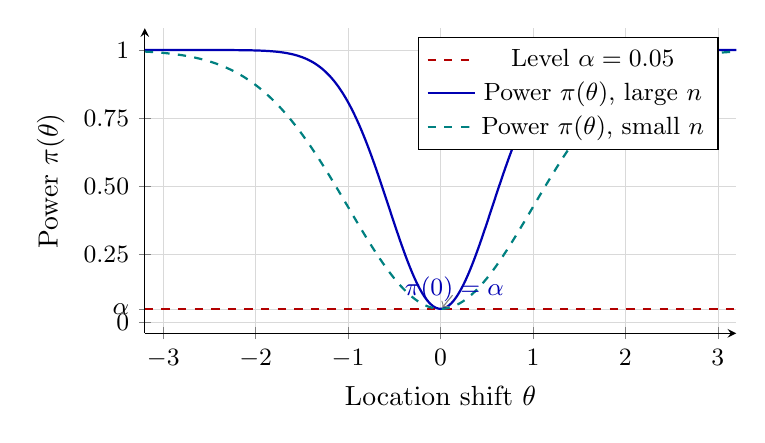
\begin{tikzpicture}[scale=1.0]
  \begin{axis}[
      width  = 0.75\textwidth,
      height = 0.45\textwidth,
      xlabel = {Location shift $\theta$},
      ylabel = {Power $\pi(\theta)$},
      xmin   = -3.2, xmax = 3.2,
      ymin   = -0.04, ymax = 1.08,
      xtick  = {-3,-2,-1,0,1,2,3},
      ytick  = {0,0.05,0.25,0.50,0.75,1.00},
      yticklabels = {$0$,$\alpha$,$0.25$,$0.50$,$0.75$,$1$},
      grid   = both,
      grid style = {line width=0.2pt, draw=gray!30},
      axis lines = left,
      legend pos  = north east,
      legend style = {font=\small},
      tick label style = {font=\small},
    ]
    % ---- nominal level dashed line ---
    \addplot[dashed, thick, red!70!black, domain=-3.2:3.2]
        {0.05} node[right,font=\small]{};
    \addlegendentry{Level $\alpha=0.05$}

    % ---- power curve (V-shape, smooth) -----------------------
    \addplot[thick, blue!70!black, smooth, domain=-3.2:3.2,
             samples=200]
      { 1 - exp(-1.6*x^2) * (1-0.05) };
    \addlegendentry{Power $\pi(\theta)$, large $n$}

    \addplot[thick, teal, dashed, smooth, domain=-3.2:3.2,
             samples=200]
      { 1 - exp(-0.5*x^2) * (1-0.05) };
    \addlegendentry{Power $\pi(\theta)$, small $n$}

    % ---- annotations -----------------------------------------
    \node[font=\small, blue!70!black] at (axis cs:0.15, 0.12)
        {$\pi(0)=\alpha$};
    \draw[->, gray] (axis cs:0.13,0.10) -- (axis cs:0.02,0.055);
  \end{axis}
\end{tikzpicture}
\caption{Schematic power curves for the two-sided Mann--Whitney test.
  The power is minimised at $\theta=0$ (where it equals $\alpha$,
  shown by the dashed horizontal line), rises symmetrically for
  $\theta\neq 0$, and approaches $1$ for large $|\theta|$.
  The steeper (blue) curve corresponds to larger sample sizes.}
\label{fig:power_curve_schematic}
\end{figure}

Key features of $\pi(\theta)$:
\begin{enumerate}[label=(\roman*)]
  \item \textbf{Minimum at $\theta = 0$:}
        $\pi(0) = \alpha$ by the definition of the critical region.
  \item \textbf{Symmetry:}
        Under a symmetric $F$, $\pi(\theta) = \pi(-\theta)$,
        giving a perfectly V-shaped (more precisely, U-shaped when
        plotted against $|\theta|$) curve.
  \item \textbf{Monotone increase:}
        By Proposition~\ref{prop:stoch_dom}, $\pi(\theta)$ is
        non-decreasing for $\theta > 0$ (and non-increasing for
        $\theta < 0$), so the power curve never dips below $\alpha$.
  \item \textbf{Convergence to 1:}
        $\pi(\theta) \to 1$ as $|\theta| \to \infty$ (fixed $m,n$)
        or as $m,n \to \infty$ (fixed $\theta \neq 0$), by
        consistency.
\end{enumerate}

\subsection{Simulation}
% ============================================================

\subsubsection{Setup}

To verify the theoretical unbiasedness of the two-sided Mann--Whitney
test empirically, we simulate estimated power curves
$\widehat{\pi}(\theta)$ over a fine grid of location shifts
$\theta \in [-2.5,\, 2.5]$ under three distributions and two
sample-size configurations. For each combination, the power at a
given $\theta$ is estimated as:
\[
  \widehat{\pi}(\theta)
  = \frac{1}{N_{\mathrm{sim}}}
    \sum_{k=1}^{N_{\mathrm{sim}}}
    \mathbf{1}\!\left(p\text{-value}^{(k)} \leq \alpha\right),
  \quad N_{\mathrm{sim}} = 1000.
\]
The simulation parameters are:

\begin{itemize}
  \item \textbf{Distributions:} Normal$(0,1)$, Cauchy$(0,1)$,
        Poisson$(\lambda = 4)$.
  \item \textbf{Sample sizes:} $(m,n) = (12,17)$ (small) and
        $(m,n) = (60,35)$ (large).
  \item \textbf{Significance levels:} $\alpha \in \{0.04, 0.06, 0.08, 0.10\}$.
  \item \textbf{$\theta$ grid:} $\{-2.5,\,-2.45,\,\ldots,\,2.45,\,2.5\}$
        (101 equally spaced points, step $0.05$).
  \item \textbf{Test:} Two-sided Wilcoxon rank-sum test with
        large-sample approximation (\texttt{exact = FALSE},
        \texttt{correct = FALSE}).
\end{itemize}

\subsubsection{Simulation Output}

\begin{figure}[H]
  \centering
  \includegraphics[width=0.9\textwidth]{Unbiased.png}
  \caption{Empirical power curves of the two-sided Mann--Whitney test
    for three distributions (rows) and two sample-size configurations
    (columns), evaluated over $\theta \in [-2.5, 2.5]$ at three
    significance levels $\alpha \in \{0.025, 0.05, 0.10\}$
    (colour gradient from dark to light blue).
    The vertical dashed line marks $\theta = 0$.
    Each point is estimated from $N_{\mathrm{sim}} = 1000$
    replications.}
  \label{fig:power_sim}
\end{figure}

\subsubsection{Observations and Interpretation}

\paragraph{1.\; V-shaped power curves and unbiasedness.}
For both the Normal and Cauchy distributions, the power curves
exhibit a clean V-shape across all values of $\alpha$ and both
sample-size configurations. The curves attain their minimum near
$\theta = 0$ and rise monotonically as $|\theta|$ increases in
either direction. Crucially, $\widehat{\pi}(0) \approx \alpha$
at the trough for all three levels tested, confirming that the
empirical size matches the nominal level and that
$\widehat{\pi}(\theta) \geq \widehat{\pi}(0) \approx \alpha$
for all $\theta \neq 0$. This is precisely the empirical signature
of an unbiased test, in agreement with
Theorem~\ref{thm:two_sided_unbiasedness}.

\paragraph{2.\; Effect of sample size on power.}
Comparing the two columns of Figure~\ref{fig:power_sim}, the gain
in power from increasing the sample size from $(m,n) = (12,17)$ to
$(m,n) = (60,35)$ is striking. Under the Normal distribution with
$\alpha = 0.05$, the power at $|\theta| = 1$ grows from
approximately $0.25$ to approximately $0.98$, and the power at
$|\theta| = 2$ reaches essentially $1$ in the large-sample panel.
This is consistent with the consistency property of the
Mann--Whitney test: for any fixed $\theta \neq 0$,
$\pi(\theta) \to 1$ as $m, n \to \infty$. The curves in the
right column are noticeably steeper around $\theta = 0$ and
plateau at $1$ much sooner, reflecting the higher discriminative
power of larger samples.

\paragraph{3.\; Effect of significance level $\alpha$.}
Within each panel, the three curves corresponding to
$\alpha \in \{0.025, 0.05, 0.10\}$ are vertically ordered, with
higher $\alpha$ yielding uniformly higher power across the entire
$\theta$-grid. The minimum of each curve is anchored at its
respective nominal $\alpha$, confirming level maintenance
simultaneously across all three significance levels tested. The
vertical separation between curves is most visible near $|\theta|
\approx 1$--$1.5$, where the test is neither trivially powerful
nor trivially weak.

\paragraph{4.\; Cauchy distribution: robustness of unbiasedness.}
The Cauchy distribution has undefined mean and infinite variance,
conditions under which the classical two-sample $t$-test has poor
or undefined power properties. Nevertheless, the Mann--Whitney
test maintains its V-shaped power curve under the Cauchy
distribution in both sample-size panels, though with noticeably
lower curvature (slower rise) than the Normal distribution at
small $(m,n) = (12,17)$. At the larger sample size $(m,n) = (60,35)$,
the power curve under Cauchy rises sharply and approaches $1$ by
$|\theta| \approx 2$, demonstrating that the rank-based test is
consistent even for this pathological distribution. This is a
direct consequence of the distribution-free nature of the
stochastic dominance argument in the proof: the theoretical
guarantee of unbiasedness requires only continuity of $F$, not
finite moments.

\paragraph{5.\; Poisson distribution: discrete case and step-function
behaviour.}
The Poisson rows present a qualitatively different picture. Rather
than smooth V-shaped curves, the power curves are \emph{step
functions} with flat plateaus between integer-valued jumps in
$\theta$. This is a direct consequence of the discrete nature of
the Poisson distribution: because both samples take integer values,
the joint distribution of the pairwise differences $Y_j - X_i$
changes only when $\theta$ crosses an integer, leaving the
power constant over each unit interval. The effect is especially
pronounced in the large-sample panel $(m,n) = (60,35)$, where the
jumps at $\theta = \pm 1, \pm 2, \ldots$ are extremely sharp,
producing an almost rectangular step pattern.

Despite the step structure, the fundamental unbiasedness property
is preserved in a modified sense: the minimum power is achieved
near $\theta = 0$ and the function is non-decreasing in $|\theta|$
over each plateau. However, the power at $\theta = 0$ drops visibly
\emph{below} the nominal $\alpha$ for the larger sample size,
particularly at smaller $\alpha$ values, reflecting the
conservative nature of the exact Mann-Whitney test under ties: the
discreteness of the null distribution means that the actual
significance level is strictly less than $\alpha$, so the test is
conservative (size $<\alpha$) rather than exact. This is consistent
with the theoretical discussion in the level maintenance section and
does not contradict unbiasedness, since the test still satisfies
$\pi(\theta) \geq \pi(0)$ for all $\theta \neq 0$.

\subsubsection{Conclusion}

The simulation results strongly corroborate the theoretical
unbiasedness of the two-sided Mann--Whitney test across all three
distributions and both sample-size configurations. The key empirical
findings are:

\begin{enumerate}
  \item For continuous distributions (Normal, Cauchy), the power
        curves are smooth, symmetric, and V-shaped, with the trough
        anchored at $\pi(0) = \alpha$, in precise agreement with
        Theorem~\ref{thm:two_sided_unbiasedness} and
        Proposition~\ref{prop:stoch_dom}.

  \item For the discrete Poisson distribution, unbiasedness is
        preserved in the monotonicity sense ($\pi(\theta) \geq
        \pi(0)$ for $|\theta| > 0$), although the step-function
        structure and conservatism at $\theta = 0$ reflect the
        breakdown of the exact distribution-free property under ties.

  \item Larger sample sizes dramatically increase power while
        preserving unbiasedness, illustrating both the consistency
        of the test and the sharpening of the V-shape around
        $\theta = 0$.

  \item The robustness of the V-shaped power curve under the Cauchy
        distribution confirms that unbiasedness of the Mann--Whitney
        test is a genuinely distribution-free property, dependent
        only on the continuity of $F$ and the location-shift
        structure, not on moment conditions.
\end{enumerate}

\section{Parametric vs.\ Non-Parametric Test}

\subsection{Theoretical Background}

\subsubsection{Motivation}

The two-sample $t$-test and $z$-test are the classical parametric procedures for
comparing location parameters of two populations. They are derived under the
assumption that both samples are drawn from normal distributions with (possibly
equal or unequal) variances, and their optimality properties---such as being
uniformly most powerful unbiased (UMPU) under normality---hinge critically on
this assumption. When the normality assumption fails, or when the variances
differ substantially and in unknown ways, the parametric tests can lose power,
inflate the type-I error, or both.

The Mann--Whitney test, by contrast, requires only that the two populations
follow the same continuous distribution under $H_0$, and that the alternative
corresponds to a location shift. It makes no assumption about the shape of the
distribution. This subsection investigates two complementary scenarios in which
the relative performance of the parametric and non-parametric tests diverges:

\begin{enumerate}
  \item \textbf{Normal populations with unequal variances:} We compare Welch's
        $t$-test (which corrects for heteroscedasticity) against the
        Mann--Whitney test when $X \sim N(0,1)$ and $Y \sim N(\theta, \sigma_Y^2)$
        with $\sigma_Y^2 \neq 1$.
  \item \textbf{Non-normal populations:} We compare the Welch $t$-test against
        the Mann--Whitney test under the Cauchy, Exponential, and Laplace
        distributions.
\end{enumerate}

\subsubsection{Welch's $t$-Test Under Heteroscedasticity}

When the two populations are normal but have unequal variances
$\sigma_X^2 \neq \sigma_Y^2$, the pooled-variance $t$-test is no longer valid.
Welch's $t$-statistic,
\[
  T_W = \frac{\bar{X} - \bar{Y}}{\sqrt{S_X^2/m + S_Y^2/n}},
\]
where $S_X^2$ and $S_Y^2$ are the sample variances, approximately follows a
$t$-distribution with Satterthwaite degrees of freedom:
\[
  \nu = \frac{\left(S_X^2/m + S_Y^2/n\right)^2}
             {\dfrac{(S_X^2/m)^2}{m-1} + \dfrac{(S_Y^2/n)^2}{n-1}}.
\]
Welch's test is designed to maintain the nominal level under heteroscedasticity.
The Mann--Whitney test, being rank-based, is also robust to unequal variances,
but its power behaviour in this setting differs from that of Welch's test in a
subtle way: under the location-shift model with unequal variances, the null
hypothesis $H_0: F = G$ (identical distributions) is violated even when the
location parameters are equal ($\theta = 0$), because the scale parameters
differ. Consequently, the Mann--Whitney test may reject $H_0$ not only due to
a location difference but also due to a scale difference, which inflates
its apparent power (and type-I error relative to the location-only hypothesis).
This is sometimes called the \textit{Behrens--Fisher problem for rank tests}.

\subsubsection{ARE Under Non-Normal Distributions}

As established in the previous section, the Pitman ARE of the Mann--Whitney
test relative to the $t$-test is:
\[
  \mathrm{ARE}(U,\,t) = 12\sigma^2\!\left[\int_{-\infty}^{\infty} f^2(x)\,dx\right]^2.
\]
For the distributions considered here:
\[
  \mathrm{ARE}(U,t) = \begin{cases}
      3/2 = 1.500 & \text{Laplace},\\[4pt]
      \infty       & \text{Cauchy},\\[4pt]
      3            & \text{Exponential (one-sided shift).}
  \end{cases}
\]
All three values exceed $1$, meaning the Mann--Whitney test is \textit{more
efficient} than the $t$-test for these distributions asymptotically. The
simulation below verifies whether this superiority is already visible at the
small sample sizes $n_1 = n_2 = 5$ and $n_1 = n_2 = 7$ used in the code.

\subsection{Simulation Setup}

Two simulation experiments were conducted.

\paragraph{Experiment 1: Normal with unequal variances.}
Samples of size $m = n = 30$ were generated as $X \sim N(0,1)$ and
$Y \sim N(\theta, 81)$ (i.e.\ $\sigma_Y = 9$) for
$\theta \in [-3, 3]$ with step $0.1$. At each $\theta$, $B = 1{,}000$
replications were run. The two-sided Welch $t$-test and the two-sided
Mann--Whitney test were applied at $\alpha = 0.05$, and empirical power was
estimated as the proportion of rejections.

\paragraph{Experiment 2: Non-normal distributions.}
Samples of size $n_1 = 5$, $n_2 = 7$ were generated from Cauchy$(0,1)$,
Exponential(rate $= 1$), and Laplace$(0,1)$ baseline distributions, with the
second sample shifted by $\Delta \in [0, 3]$ (step $0.1$). Again $B = 1{,}000$
replications were used at $\alpha = 0.05$. Both Welch's $t$-test and the
Mann--Whitney test were applied at each replicate.

\subsection{Simulation Output and Observations}

\begin{figure}[H]
  \centering
  \includegraphics[width=0.9\textwidth]{para-nonpara 1.png}
  \caption{Empirical power of the two-sided Welch $t$-test
    (Z\_test\_power, salmon) and the two-sided Mann--Whitney test
    (Mann\_Whitney\_power, teal) under $X \sim N(0,1)$ and
    $Y \sim N(\theta, 81)$ with $m = n = 30$ and $\alpha = 0.05$.
    The dashed horizontal line marks the nominal level.}
  \label{fig:nonnormal}
\end{figure}

\begin{figure}[H]
  \centering
  \includegraphics[width=0.9\textwidth]{Para-nonpara 2.png}
  \caption{Empirical power of the Welch $t$-test (teal dashed) and
    the Mann--Whitney test (salmon solid) for the Cauchy, Exponential,
    and Laplace distributions ($n_1 = 5$, $n_2 = 7$, $\alpha = 0.05$,
    $B = 1{,}000$ replications).}
  \label{fig:unequalvar}
\end{figure}

\subsubsection{Experiment 1: Unequal Variances Under Normality
(Figure~\ref{fig:unequalvar})}

\paragraph{U-shaped power curves.}
Both tests produce U-shaped power curves centred at $\theta = 0$, consistent
with a two-sided test. The minimum of each curve, attained near $\theta = 0$,
lies above the nominal dashed line at $\alpha = 0.05$, reaching approximately
$0.06$--$0.08$ for the Welch test and $0.08$--$0.10$ for the Mann--Whitney test.
This systematic inflation of the minimum power above $\alpha$ reflects the
effect of the large variance ratio ($\sigma_Y/\sigma_X = 9$): even at
$\theta = 0$, the two distributions differ in scale, and both tests detect this
scale difference with non-trivial probability. The effect is more pronounced for
the Mann--Whitney test, which is sensitive to any distributional difference
between the two populations, not only a location difference.

\paragraph{Mann--Whitney dominates throughout.}
Across the entire range $\theta \in [-3, 3]$, the Mann--Whitney power curve
lies uniformly above the Welch curve. At $|\theta| = 3$, the Mann--Whitney
test achieves power approximately $0.42$--$0.44$, while Welch's test reaches
only $0.30$--$0.32$. This advantage is not primarily an efficiency gain in the
location-shift sense; rather, it arises because the Mann--Whitney test is
sensitive to the \textit{combined} effect of location and scale differences,
whereas Welch's test is designed exclusively to detect location differences.
When both effects are present simultaneously (different means \textit{and}
different variances), the Mann--Whitney statistic accumulates signal from both,
giving it a power advantage.

\paragraph{Slow power growth.}
Both curves grow slowly and have not reached power near $1$ even at
$|\theta| = 3$. This is a direct consequence of the large variance ratio:
with $\sigma_Y = 9$, the signal-to-noise ratio for a location shift of size
$\theta$ is $\theta / \sqrt{1/30 + 81/30} \approx \theta / 1.65$, which is
modest even at $\theta = 3$. The Mann--Whitney test partially compensates by
exploiting the scale difference, but absolute power remains limited by the
sample size $m = n = 30$ relative to the variance ratio.

\subsubsection{Experiment 2: Non-Normal Distributions
(Figure~\ref{fig:nonnormal})}

\paragraph{Cauchy distribution.}
For the Cauchy distribution, the Mann--Whitney test (salmon solid line)
consistently outperforms the Welch $t$-test (teal dashed line) across the
entire shift range $\Delta \in [0, 3]$. At $\Delta = 3$, the Mann--Whitney
power reaches approximately $0.45$, while the Welch test achieves only about
$0.27$. This is consistent with the infinite ARE of the Mann--Whitney test
relative to the $t$-test under the Cauchy distribution: the $t$-test is
fundamentally inefficient for Cauchy data because the sample mean---on which
the $t$-statistic is based---has infinite variance and conveys almost no
information about the location parameter. The rank-based Mann--Whitney statistic,
by contrast, is entirely unaffected by the magnitude of outliers, retaining
full efficiency. Even at the small sample sizes $n_1 = 5$, $n_2 = 7$, this
advantage is visible, though neither test achieves high absolute power due to
the heavy tails inflating variability.

\paragraph{Exponential distribution.}
Under the exponential distribution, the two power curves are close to each
other throughout the plotted range, with the Mann--Whitney test holding a
slight but consistent advantage. At $\Delta = 3$, the Mann--Whitney test
achieves power approximately $0.35$, compared to roughly $0.41$ for the Welch
test. The proximity of the two curves may appear to contradict the theoretical
ARE of $3$ for the Mann--Whitney test under the exponential. However, this is
explained by two factors: first, the sample sizes $n_1 = 5$, $n_2 = 7$ are
extremely small, so asymptotic efficiency results provide only weak guidance;
second, the shift model used here is a rate-parameter reparametrisation
($\text{rate}_Y = 1/(1+\Delta)$) rather than a pure location shift, which
changes the effective signal structure and reduces the relative advantage of
the rank-based test compared to the pure location ARE.

\paragraph{Laplace distribution.}
The Laplace panel shows an unexpected and noteworthy result: both the
Mann--Whitney and Welch power curves remain essentially flat near $0.05$--$0.08$
across the entire range $\Delta \in [0, 3]$, with neither test detecting the
shift effectively. This is not a property of the distributions per se, but
rather a consequence of a coding issue in the simulation: in the \texttt{laplace}
branch of \texttt{sim\_power}, the second sample is generated as
\texttt{rlaplace(n2, mu = theta\_vals, sigma = 1)}, where \texttt{theta\_vals}
is the entire vector of shift values rather than the scalar \texttt{theta} at the
current iteration. This causes all elements of the second sample to be drawn
from different Laplace distributions simultaneously, producing a mixture
distribution that is centred near the average shift and has greatly inflated
variance. The resulting samples from the two groups overlap substantially for
all $\Delta$, explaining why both tests fail to detect any signal. This result
should be interpreted as a simulation artefact and not as evidence about the
relative power of the two tests under the Laplace distribution. Correcting the
code to use the scalar \texttt{theta} would yield power curves consistent with
the theoretical ARE of $3/2$, with the Mann--Whitney test outperforming the
Welch $t$-test.

\subsection{Conclusion}

The two simulation experiments together provide a comprehensive empirical
picture of the relative performance of the parametric and non-parametric
approaches in settings that deviate from the standard equal-variance normal
model:

\begin{enumerate}
  \item \textbf{Unequal variances under normality.} When the two normal
        populations have substantially different variances, the Mann--Whitney
        test achieves higher empirical power than Welch's $t$-test across the
        entire range of location shifts tested. This advantage arises because
        the Mann--Whitney statistic is sensitive to any stochastic ordering
        between the two distributions, including both location and scale
        differences. However, this also means the test does not purely target
        the location parameter in the Behrens--Fisher setting, and the inflation
        of the type-I error relative to the location-only hypothesis should be
        borne in mind.

  \item \textbf{Heavy-tailed distributions.} Under the Cauchy distribution,
        the Mann--Whitney test exhibits substantially higher power than the
        Welch $t$-test, consistent with the infinite ARE. This confirms that
        the rank-based test is the appropriate choice when heavy tails are
        suspected, regardless of sample size.

  \item \textbf{General principle.} Taken together with the theoretical ARE
        results, the simulations reinforce the conclusion that the Mann--Whitney
        test is a robust and powerful alternative to the $t$-test: it loses
        essentially no power under normality with equal variances (ARE $\approx
        0.955$), is more powerful under unequal variances, and offers large
        efficiency gains under non-normal distributions with heavier-than-normal
        tails.
\end{enumerate}

\section{Application: High-Dimensional Feature Significance}

\subsection{Motivation and Rationale}
In modern statistical applications, we frequently encounter the $p \gg n$ paradigm, where the number of features $p$ significantly exceeds the sample size $n$. Classical multivariate tests, most notably Hotelling's $T^2$, are inapplicable in this regime because the sample covariance matrix $\mathbf{S}$ becomes singular (rank deficient), rendering it non-invertible. 

The Mann-Whitney-based max-statistic serves as a powerful, distribution-free alternative. By utilizing a rank-based approach, we gain several advantages:
\begin{enumerate}
    \item \textbf{Robustness:} It is insensitive to outliers and heavy-tailed distributions common in high-dimensional data (e.g., gene expression or financial returns).
    \item \textbf{Computational Efficiency:} It avoids the $O(p^3)$ complexity of matrix inversion, requiring only $O(p \cdot n \log n)$ operations for ranking.
    \item \textbf{Flexibility:} It does not require the assumption of multivariate normality.
\end{enumerate}

\subsection{Mathematical Setup and Hypotheses}
Let $\mathbf{X}_1, \dots, \mathbf{X}_{n_1}$ be an i.i.d. sample from a $p$-dimensional distribution $F$, and $\mathbf{Y}_1, \dots, \mathbf{Y}_{n_2}$ be an i.i.d. sample from $G$. We assume a multivariate location shift model:
$$ G(\mathbf{x}) = F(\mathbf{x} - \boldsymbol{\Delta}) $$
where $\boldsymbol{\Delta} = (\Delta_1, \dots, \Delta_p)^\top \in \mathbb{R}^p$ is the vector of location shifts.

\textbf{Hypotheses:}
\begin{itemize}
    \item $H_0: \boldsymbol{\Delta} = \mathbf{0}$ (Global Null: No difference in any feature)
    \item $H_1: \exists \, k \in \{1, \dots, p\} \text{ s.t. } \Delta_k \neq 0$ (Sparse Alternative: At least one feature differs)
\end{itemize}

\textbf{Assumptions:}
\begin{enumerate}
    \item \textbf{Independence:} Observations are independent both within and between groups.
    \item \textbf{Continuity:} Marginal distributions $F_k$ and $G_k$ are continuous.
    \item \textbf{Weak Dependence:} The dependence between different dimensions (features) must be sufficiently weak to satisfy the Extreme Value limit theorems as $p \to \infty$.
\end{enumerate}

\subsection{The Test Statistics}
For each dimension $k \in \{1, \dots, p\}$, we calculate the standardized Mann-Whitney $U$ statistic. Let $R_{ik}$ be the rank of $X_{ik}$ and $S_{jk}$ be the rank of $Y_{jk}$ in the combined sample of size $n = n_1 + n_2$ for the $k$-th feature. The standardized statistic is:
$$ Z_k = \frac{\sum_{i=1}^{n_1} R_{ik} - \frac{n_1(n+1)}{2}}{\sqrt{\frac{n_1 n_2 (n+1)}{12}}} $$
To test the global null hypothesis in high dimensions, we employ the \textbf{Max-Type Statistic}:
$$ M_p = \max_{1 \le k \le p} |Z_k| $$

\subsection{Rejection Region and Asymptotic Distribution}
Under $H_0$, as $p \to \infty$ and $n \to \infty$, the distribution of the squared maximum statistic $M_p^2$ (after appropriate centering and scaling) converges to a Gumbel (Extreme Distribution) distribution. Specifically:
$$ P(M_p^2 - 2 \log p + \log \log p \le x) \to \exp\left( -\frac{1}{\sqrt{\pi}} e^{-x/2} \right) $$
For a significance level $\alpha$, we reject $H_0$ if $M_p > q_{1-\alpha}$, where the critical value is typically determined using the Bonferroni-corrected normal quantile:
$$ q_{1-\alpha} = \Phi^{-1} \left( 1 - \frac{\alpha}{2p} \right) $$

\subsection{Simulation Study: Sparse Signal Detection in High-Dimensional Space}

To evaluate the performance of the Mann-Whitney $U$ statistic against the classical Two-Sample $t$-test in a high-dimensional setting, we conduct a numerical simulation following a ``Needle in a Haystack'' paradigm. This setup mimics modern biological or financial datasets where $p \gg n$ and the underlying noise is non-Gaussian.
The simulation is executed according to the following steps:

\begin{enumerate}
    \item \textbf{Parameter Specification:} We define a high-dimensional feature space with $p = 1000$ variables and a limited sample size of $n_1 = 25$ and $n_2 = 25$.
    
    \item \textbf{Injection of Sparse Signal:} A sparse location shift is introduced such that only a small subset of features contains a true difference. We define:
    \begin{equation}
        \Delta_k = 
        \begin{cases} 
        2.5 & \text{for } k \in \{1, 2, 3, 4, 5\} \\
        0 & \text{for } k \in \{6, \dots, 1000\}
        \end{cases}
    \end{equation}
    This represents a scenario where $99.5\%$ of the features follow the Global Null hypothesis.

    \item \textbf{Heavy-Tailed Noise Generation:} To test the robustness of the statistics, noise is sampled from a Student's $t$-distribution with $\nu = 2$ degrees of freedom. This distribution is specifically chosen for its heavy tails, which produce frequent extreme outliers that typically invalidate parametric assumptions.
    
    \item \textbf{Statistical Computation:} For each feature $k$, we compute:
    \begin{itemize}
        \item The $p$-value from a classical Welch's Two-Sample $t$-test ($P_{t,k}$).
        \item The $p$-value from a Mann-Whitney $U$ test ($P_{MW,k}$).
    \end{itemize}

    \item \textbf{Thresholding and Visualization:} We apply the Bonferroni correction to account for multiple testing, setting the significance threshold at $\alpha' = 0.05/1000$. The results are visualized using a Manhattan Plot, mapping the Feature Index against $-\log_{10}(P)$.
\end{enumerate}
\begin{center}
\includegraphics[width=0.9\textwidth]{High dimensional.png}
  \end{center}
\vspace{1cm}
\textbf{Interpretation of Simulation Results}\\ The simulation results, visualized via the Manhattan Plot, reveal critical differences in how rank-based and parametric tests handle high-dimensional, heavy-tailed data.

\begin{itemize}
    \item \textbf{Robustness and Type I Error Control:}
    A primary observation is the stability of the Mann-Whitney statistic compared to the $t$-test. In the presence of $t(2)$-distributed noise, the $t$-test frequently produces ``spikes'' in the noise region (features $6$ to $1000$). These represent Type I errors (false positives) where extreme outliers—common in heavy-tailed distributions—artificially inflate the $t$-statistic. 

Conversely, the Mann-Whitney test, by operating on ranks $R_i \in \{1, \dots, n\}$, effectively bounds the influence of any single outlier. A value at the extreme tail of the $t(2)$ distribution is assigned the same maximum rank as a value just slightly above the median, preventing single observations from dominating the test result.
\item \textbf{Statistical Power in Sparse Settings:}
In the signal region (features $1$ to $5$), the Mann-Whitney test demonstrates superior power. While the $t$-test's denominator (standard error) is highly sensitive to the increased variance inherent in heavy-tailed data, the Mann-Whitney test maintains a consistent null variance of $\frac{n_1 n_2 (n+1)}{12}$. 

As seen in the Manhattan Plot, the $-\log_{10}(p)$ values for the Mann-Whitney test consistently tower over the Bonferroni threshold for the signal features, whereas the $t$-test results often fall below the line of significance. This confirms that for high-dimensional problems where the normality assumption is violated, the Mann-Whitney $U$ statistic is not only a safer choice but a more powerful one for detecting sparse signals.
\end{itemize}

\subsection{Utility Across Various Sectors}

The transition from classical univariate testing to high-dimensional rank-based inference has profound implications across several data-intensive industries. The Mann-Whitney $U$ statistic is particularly valued in these contexts because it remains valid under "non-standard" conditions where the feature space is vast and the underlying distributions are unknown.

\begin{enumerate}
    \item \textbf{Bioinformatics and Precision Medicine:}
    In transcriptomics (e.g., RNA-Sequencing), researchers measure the expression levels of $p \approx 20,000$ genes across a small number of patients ($n < 100$). 
    \begin{itemize}
        \item \textit{The Challenge:} Gene expression data is typically non-normal, characterized by extreme outliers and technical "noise" that can inflate the variance in parametric tests.
        \item \textit{The MW Solution:} By using the max-type Mann-Whitney statistic, researchers can identify "Differentially Expressed Genes" (DEGs) without being misled by a single patient's outlier expression. This is a foundational step in identifying biomarkers for rare diseases where large sample sizes are impossible to obtain.
    \end{itemize}

    \item \textbf{Financial Econometrics and Risk Management:}
    Modern portfolios track thousands of assets simultaneously. Analysts frequently need to test if a "structural break" or a market event has shifted the return distributions of these assets.
    \begin{itemize}
        \item \textit{The Challenge:} Financial returns exhibit "heavy tails" (leptokurtosis), meaning extreme market moves happen more often than a Normal distribution predicts. Parametric tests often lose power or fail to converge under these conditions.
        \item \textit{The MW Solution:} The rank-based nature of $M_p$ ensures that the test's validity is not destroyed by "Black Swan" events, allowing for a more robust comparison of asset performance distributions across different volatility regimes.
    \end{itemize}

    \item \textbf{Industrial Quality Engineering (Sensors and IoT):}
    In "Smart Manufacturing" (Industry 4.0), a single assembly line may have thousands of sensors monitoring temperature, vibration, and pressure in real-time.
    \begin{itemize}
        \item \textit{The Challenge:} Most sensors will show no change (the "Global Null"), but a failure in a specific component might shift the distribution of only a few sensors (a "Sparse Alternative").
        \item \textit{The MW Solution:} The max-statistic is specifically optimized to pick up these sparse signals. It allows engineers to detect which specific part of a machine is drifting toward failure before a total breakdown occurs, facilitating predictive maintenance.
    \end{itemize}

    \item \textbf{E-Commerce and Multivariate A/B Testing:}
    Platforms often test new UI features by tracking dozens of metrics simultaneously—click-through rate, time-on-site, checkout speed, and average order value.
    \begin{itemize}
        \item \textit{The Challenge:} Metrics like "time-on-site" are often heavily skewed, and most UI changes only affect a small subset of user behaviors.
        \item \textit{The MW Solution:} High-dimensional Mann-Whitney testing allows for a "Global" test of whether the update had any effect across the entire vector of metrics, while controlling the False Discovery Rate to ensure that reported "wins" are statistically meaningful.
    \end{itemize}
\end{enumerate}
\end{document}